% arara: pdflatex
% arara: pdflatex
% arara: pdflatex

% options:
% thesis=B bachelor's thesis
% thesis=M master's thesis
% czech thesis in Czech language
% slovak thesis in Slovak language
% english thesis in English language
% hidelinks remove colour boxes around hyperlinks

\documentclass[thesis=B,czech]{template/FITthesis}[2019/12/23]

\usepackage[utf8]{inputenc} % LaTeX source encoded as UTF-8

% \usepackage{amsmath} %advanced maths
% \usepackage{amssymb} %additional math symbols

\usepackage{dirtree} %directory tree visualisation
\usepackage{biblatex}
\usepackage{csquotes}
\usepackage{xevlna}
\usepackage{graphics}
\addbibresource{template/mybibliographyfile.bib}


% list of acronyms
% \usepackage[acronym,nonumberlist,toc,numberedsection=autolabel]{glossaries}
% \iflanguage{czech}{\renewcommand*{\acronymname}{Seznam pou{\v z}it{\' y}ch zkratek}}{}
% \makeglossaries


\newcommand{\tg}{\mathop{\mathrm{tg}}} %cesky tangens
\newcommand{\cotg}{\mathop{\mathrm{cotg}}} %cesky cotangens

% % % % % % % % % % % % % % % % % % % % % % % % % % % % % % 
% ODTUD DAL VSE ZMENTE
% % % % % % % % % % % % % % % % % % % % % % % % % % % % % % 

% \title {Serverový backend Android aplikace pro podporu rodin v rozvodovém řízení}
% \authorGN {Iaroslav}
% \authorFN {Kolodka}
% \authorWithDegrees {Iaroslav Kolodka}
% \author {Iaroslav Kolodka}
% \supervisor {Ing. Jiří Hunka}
% \keywordsCS {backend}
% \keywordsEN {backend}
% \department {Katedra softwarového inženýrství}
% \placeForDeclarationOfAuthenticity {V~Praze}
% \declarationOfAuthenticityOption {4}
% \website {https://gitlab.fit.cvut.cz/kolodiar/bp-thesis}
% \assignment{pdfs/assignment.pdf}

\department{Katedra softwarového inženýrství}
\title{Serverový backend Android aplikace pro podporu rodin v rozvodovém řízení}
\authorGN{Iaroslav} %(křestní) jméno (jména) autora
\authorFN{Kolodka} %příjmení autora
\authorWithDegrees{Iaroslav Kolodka} %jméno autora včetně současných akademických titulů
\author{Iaroslav Kolodka} %jméno autora bez akademických titulů
\supervisor{Ing. Jiří Hunka}
\acknowledgements{Rád bych poděkoval všem lidem, bez kterých tato práce by nemohla vzniknout. Hlavně bych chtěl poděkovat vedoucímu práce - Ing. Jiřího Hunku, který vždycky měl čas na moudrou rádu. Také důležité poděkování manažer tohoto - Oldovi Malcovi - projektu, který vždycky měl čas na pomoc, kdy jsem měl jakýkoliv problém. Zvláštní poděkování patři mému kolegovi - Martinu Beranu, který současně pracoval na frontdendu aplikace. Díky práce Martina jsem měl zpětnou vazbu, jakou funkcionalitu mám přidat a jakou mám předělat.}
\abstractCS{Tato bakalářská práce se zabývá realizací serverového backendu Android aplikace pro podporu rodin v rozvodovém řízení včetně. Implementace se provádí na základě již existujícího návrhu, který byl proveden v rámci předmětů BI-SP1\footnote{Softwarový týmový projekt 1} a BI-SP2\footnote{Softwarový týmový projekt 2} bakalářského studia vyučovaných na FIT ČVUT, které se zúčastnil autor teto práci. Pro dosažení lepšího výsledků byly navěny vhodné úpravy podle požadavků frontedové častí aplikace, kterou se zabývá kolega - Martin Beran - v souběžné bakalářské práce. Backend aplikace, který je předmětem teto práci, je napsán v jazyce Kotlin. Pro návrh REST API byl zvolen framework Spring. Pro testování aplikace byly zvoleny frameworky JUnit 5 a funkcionalita, kterou poskytuje framework Spring. Za účely návrhu bezpečnosti server využívá protokoly HTTPS a OAuth 2.0 . Pro dokumentace REST API byl zvolen framework Swagger. Byly navrženy vhodné budoucí kroky, které budou implementovány po dokončení teto bakalářské práce.}
% \abstractCS{V~několika větách shrňte obsah a přínos této práce v~češtině. Po přečtení abstraktu by se čtenář měl mít čtenář dost informací pro rozhodnutí, zda chce Vaši práci číst.}
\abstractEN{This bachelor's thesis deals with the implementation of a server backend Android application to support families in divorce proceedings, including. The implementation is carried out on the basis of an existing proposal, which was carried out within the subjects BI-SP1\footnote{Team Software Projket 1} and BI-SP2\footnote{Team Software Projekt 2} of the bachelor's study taught at FIT CTU, which was attended by the author of this work. The application design was modified according to the requirements of the fronted part of the application to achieve better results, which is developing by a colleague - Martin Beran - in a parallel bachelor's work. The backend application, which is the subject of this work, is written in the Kotlin language. The Spring framework was chosen to design the REST API. The JUnit 5 frameworks and the functionality provided by the Spring framework were chosen to test the application. For security design purposes, the server uses the HTTPS and OAuth 2.0 protocols. The Swagger framework was chosen for the REST API documentation. Appropriate future steps have been proposed and will be implemented after the completion of this bachelor thesis.}
% \abstractEN{Sem doplňte ekvivalent abstraktu Vaší práce v~angličtině.}
\placeForDeclarationOfAuthenticity{V~Praze}
\declarationOfAuthenticityOption{4} %volba Prohlášení (číslo 1-6)
\keywordsCS{Serverový backend, Kotlin, REST, API, Spring}
\keywordsEN{Server backend, Kotlin, REST, API, Spring}
\website{https://gitlab.fit.cvut.cz/kolodiar/bp-thesis} %volitelná URL práce, objeví se v tiráži - úplně odstraňte, nemáte-li URL práce
\assignment{pdfs/assignment.pdf}
% \website{http://site.example/thesis} %volitelná URL práce, objeví se v tiráži - úplně odstraňte, nemáte-li URL práce

\begin{document}

% \newacronym{CVUT}{{\v C}VUT}{{\v C}esk{\' e} vysok{\' e} u{\v c}en{\' i} technick{\' e} v Praze}
% \newacronym{FIT}{FIT}{Fakulta informa{\v c}n{\' i}ch technologi{\' i}}

\begin{introduction}
	Všichni se během svého života setkávají s člověkem, se kterým se stávají nerozluční. Časem se přichází svatba a dětí. I když myslíme, že láska je navěky, pořad se lidé rozvádí. Většinou manžele po rozvodu chtějí co nejméně komunikovat mezi sebou. Konflikt se může vzniknout kvůli čemu-koliv. Manžele můžou nerespektovat jeden druhého nebo dokonce i dělat něco naschvál druhému. Rozvadění je těžké pro obou z manželů, ale pro dětí je tohle období daleko horší. Dětí se často stávají v teto situaci centrem konfliktu.  


Jedním ze způsobů jak odstínit dítě od konfliktu samotného je zabezpečit komunikaci manželů pomoci aplikaci,  funkcionalita které by měla pokrývat nejdůležitější aspekty které mají vliv na dítěte, což je zprava pečovatelských dnů, zprava alimentů a zprava nákupu pro dítěte. Tyto věcí brání rodičům využit dítěte jako zbraň v konfliktech mezi sebou.

Toto téma jsem vybral, protože jsem chtěl pracovat nad zajímavým reálným projektem, který v budoucnu budou lidi používat. V rámci zadání mám pracovat s moderním programovacím jazykem Kotlin. Mám rád ideologii tohoto jazyku, proto je mi příjemné pracovat nad implementací projektu.


Projekt se skládá z mobilní aplikaci, kterou souběžně řeší v rámci bakalářské práci Martin Beran, a Serverové častí, kterou řeším v rámci teto bakalářské práci. V analýze vycházím z výsledku předmětů BI-SP1 a BI-SP2. Zúčastnil jsem se obou předmětu a vystupoval jsem hlavně jako backend programátor. V rámci druhé častí softwarového projektu také jsem byl vedoucím backendového týmu.


Tato práce se skládá z pěti kapitol. První kapitola je věnovaná rešerše, Druha kapitola je určena analýze. Třetí kapitola – návrhu. Čtvrtá kapitola – Implementaci. A poslední, pátá kapitola, je věnovaná testovaní serveru.
% 	\chapter{Cíl práce}
\end{introduction}


\chapter{Rešeře}\label{resere}
\section{Kotlin}\label{resere:kotlin}
    Kotlin je relativně nový jazyk pro JVM. Poprvé tento jazyk byl představen společnosti v 2011 roku. První stabilní verze byla představena v únoru roku 2016. Ale už v květnu roku 2017 Kotlin se stal oficiálním jazykem pro Android.
    
    Kotlin byl vytvořen jako alternativa jazyku Java a řeší některé jí problémy. Například, Kotlin řeší problém použití null, také známý jako \textit{The Billion Dollar Mistake}\cite{theBDM}, a spojené s ní problémy. Java samotna nemá podporu pro \textit{not-null} proměnné, ale Kotlin takovou podporu má, a to v podobě oddělení \textit{nullable} typu pomocí ? operátoru.
    
    Kotlin je odlišný od Javy i syntaxí. Například není potřeba psát středník pro dokončeni příkazu, ale je vyžadován pouze v případe, že chcete oddělit několik příkazů na jedné řádce. Také byly odstraněny spousta klíčových slov. Například pro deklarací \textit{public final} proměnné je potřeba použit klíčově slovo \textit{val}. Důležitým rozdílem je, že při vytvoření třídy Kotlin umí vygenerovat metody \textit{get} a popřípadě i \textit{set} a umožňuje zadávat defaultní hodnoty v konstruktoru. Také Kotlin zavádí \textit{data class}, který navíc od obyčejné třídy umí vygenerovat metod \textit{toString}, který převádí třídu na typ \textit{String} v čítelné podobě \cite{Priklad vygenerovane tridy}, a metody \textit{equals} a \textit{hashCode}. Celý seznam věcí, které Kotlin má navíc od Javy nebo má jinou implementaci, což není předmětem teto práci, nemá smysl. Proto 
    
    
    Kotlin je Kotlin podporuje \textit{type-safe builder}
\section{J2EE}\label{resere:j2ee}
    
\section{Testování}\label{resere:testovani}

\chapter{Analýza}
\label{chapter:analyza}
Hlavním cílem teto bakalářské práce je implementovat návrh backendu podle návrhu a fragmentu implementace, které byly udělány v rámci předmětů BI-SP1 a BI-SP2 bakalářského studia vyučovaných na FIT ČVUT v akademickém roce 2018/2019 a 2019/2020. Tato kapitola se zabývá analýzou výsledků zmíněných předmětu. Autor práce je zároveň i absolventem těchto předmětů, kde pracoval v týmu na analýze požadavku zákazníka a pak pracoval jako backend vývojář a vedoucí backendového týmu.

Pro jasné zajištěni verze aplikace, která bude předmětem analýzy teto kapitoly, uvádím datům ukončení práce na projektu v rámci předmětu BI-SP2 - 25. února 2020. Také pro možnost pohodlně vyhledat konkretní verze uvádím poslední 
\textit{commit}\footnote{252b0288dbfe9942446b78fd452c0edce810a370} udělaný v rámci tohoto předmětu.

% Tato kapitola se zabývá popisem současného stavu aplikace, který je výsledkem zmíněných předmětů.

% Hlavním cílem teto bakalářské práce je implementovat návrh backendu podle návrhu a fragmentu implementace, které byly rozpracovány v rámci předmětů BI-SP1 BI-SP2 bakalářského studia vyučovaných na FIT ČVUT. Dalším cílem teto práci je navrhnou vhodné úpravy za účelem dosažení kvalitnějšího výsledku a splnění požadavku frontedové častí aplikace. Autor teto práci absolvoval zmíněné předměty, proto pro zajištění rozdilu v 

    \section{Analýza současného návrhu} \label{analyza:analyza navrhu}
    
     \subsection{Předmět BI-SP1}\label{analyza:navrh:sp2}
        V rámci předměty BI-SP1 pracovalo sedm lidí včetně autora teto práci. Tým měl za úkol analýz požadavku zákazníka a návrh implementaci aplikace. Aplikace se skládá ze dvou částí. Serverového backendu, který je předmětem teto bakalářské práci a frontendové častí aplikace, kterou současně v rámci bakalářské prací implementuje kolega - Martin Beran. Frontendová část aplikace je Android aplikací. Backendová část je serverovým backendém, který má poskytovat REST\footnote{Representational State Transfer} API pro Android aplikaci.
    
        Během semestru tým provedl kompletní analýzu požadavku zákazníka. Především, tým navrhl scénáře použiti aplikace:
        \begin{itemize}
	        \item Přihlašování/Registrace;
	        \item Přihlašování/Registrace do rodiny;
	        \item Role v aplikace a jejich vytváření;
	        \item Nastavení pečovatelský dnů;
	        \item Kalendář;
	        \item Kniha potřeb dítěte;
	        \item Uchování účtenek;
	        \item Správa alimentů.
        \end{itemize}
        Potom byly navrženy Use Case Diagram a Activity Diagramy, podle kterých byly navrženy Wireframy a Doménový model. 
    
        \subsection{Předmět BI-SP2}\label{analyza:navrh:sp2}
            Cílem předmětu BI-SP2 byla implementace návrhu předmětu BI-SP2. Autor teto práce pracoval v backendovém týmu a zároveň vystupoval v roli vedoucího backendového týmu.
        
            Pro vývoj backendové častí aplikace byl zvolen jazyk Kotlin, zmíněný v sekci \ref{resere:kotlin}, a framework Spring, zmíněný v sekci \ref{resere:j2ee}. Jako {buildovací system}\footnote{nástroj pro automatizaci sestavování programu} byl zvoleny nástroj Gradle. Podrobnnějí výsledky předmětu BI-SP2 probrány v sekce \ref{analyza:soucasnaImplementace}.
        
    
        \subsection{Doménový model}\label{analyza:navrh:DomainModel}
            Hlavním zdrojem informace o výsledném návrhu serveru je Doménový model. Kompletní Doménový model se nachází v příloze \ref{dodatek:DomainModel}. Zelenou barvou jsou označeny třídy, které už jsou implementovány. žlutou barvou jsou označeny třídy, které ještě nejsou implementovány. Také, jsou třídy označeny zároveň žlutou a zelenou barvou, což znamená, že třída je implementována jenom částečně. Taková situace se mohla nastat v případe, že implementace vyžadovala implementace jiné třídy, která ještě neexistovala. Tento Doménový model má určité nedostatky podle požadavku frontedové části aplikace. Jako příklad takových nedostatku je možné uvést zbytečně komplikovaný návrh Intervalů (viz. obrázek \ref{image:Interval1}), který byl od začátku předělán.

    \subsection{Registrace a přihlášeni do rodiny}
        Aplikace je navržena tak, že první uživatel, který má vytvořit svůj účet je jeden z rodičů. Pro registraci člověk potřebuje řadu povinných údajů:
        \begin{itemize}
	        \item jméno - zvolené jméno se stává jeho implicitním jménem v systému
	        \item příjmení - zvolené příjmení se stává jeho implicitním příjmením v systému
	        \item email - zvolený email je identifikátorem uživatele v rámci systému
        \end{itemize}
        Na základe těchto údajů se vytváří unikátní uživatel v rámci systému. V tomto stavu člověk není přihlášeny do žádné rodiny a nemá žádnou roli. Podrobněji role budou popsané v sekci \ref{analyza:bezpecnost:role}. \textit{User} také může mít implicitní obrázek profilu (viz. obrázek \ref{image:User-Image1}).
        \begin{figure}\centering
	        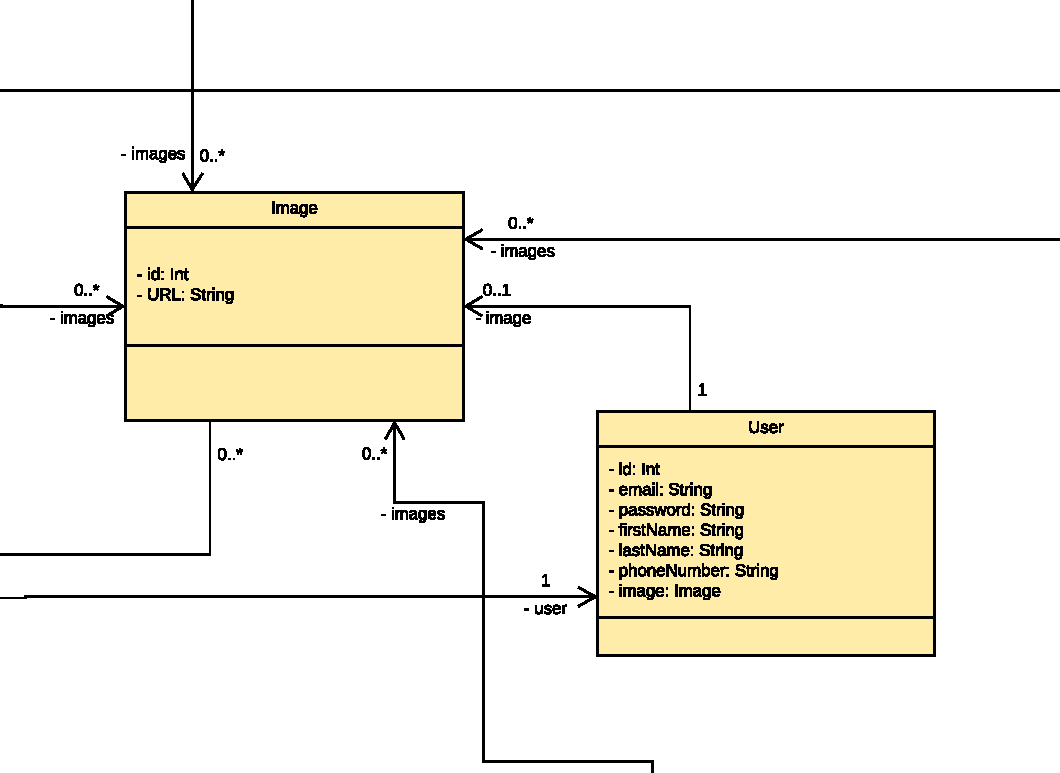
\includegraphics[width=0.5\textwidth]{pdfs/User-Image1}
	        \caption[Návrh Rolí]{Návrh třídy Role podle Doménovém modelu z předmětu BI-SP2}\label{image:User-Image1}
        \end{figure}
        
        Potom uživatel má možnost vytvořit rodinu nebo přihlásit se do již existující rodiny. Pro vytvoření nové rodiny, uživatel potřebuje zadat jméno rodiny a přidat členy rodiny. Autor teto rodiny automaticky se stává jedním s rodičů teto rodiny. jinou možností je přihlásit se do rodiny, která již existuje. Podmínkou k tomu je existování pozvání do některé existující rodiny. V takovém případě uživatel už nemá možnost zvolit role v rámci rodiny. Role má být nastavena uživatelem, který vytvořil toto pozvání.

    \subsection{Kalendář}    
        Kalendář je hlavním zdrojem informaci pro celou rodinu, který společný pro všechny uživatele. Na něm jsou zobrazené zvýrazněné různými barvami pečovatelské dny obou rodičů a důležité události, které mohou být jednorázové nebo pravidelné. 
        
        Kromě dlouhodobých nastavení pečovatelských dnu, kalendář může zobrazovat i jednorázové změny, které mohou vidět všechny členy rodiny. Takový postup pomáhá rodině eliminovat situace, kdy několik členu rodiny najednou myslí, že je v konkretní den dítě v jejích péči nebo několik členu rodiny najednou říkají, že není to jejích den.  
        
    \subsection{Alimenty}    
        Aplikace řeší i finanční problémy. Hlavní problémem jsou alimenty, které má pravidelně uhrazovat jeden z rodičů. Tento proces byl rozdělen do dvou častí. První častí je nastavení dlouhodobých pravidel pro splacení alimentů. Druhou častí jsou samotné alimenty, které se generuje na základě dlouhodobých nastavení. Jedna rodina může mít zároveň několik nastavení v případě, že jedna rodina má několik dětí nebo chce rozdělit alimenty do logický částí.
    
    \subsection{Kniha potřeb dítěte}
        Aplikace by měla pomáhat i dítěti.    
        
   
    
    \section{Analýza současné implementace}\label{analyza:soucasnaImplementace}
        Projekt má ve složce \textit{main}\footnote{bi-springboot/src/main} 69 souborů a 845 řádek kódů. Implementace částečné pokrývá Doménový model zmíněný v sekci \ref{analyza:navrh:DomainModel}. 
    
    \section{Analýza požadavku frontendu}
    
    \section{Analýza konkurence}
        Tento 
% \section{Analýza testování}

    \section{Analýza bezpečnosti}
    
        \subsection{Role}\label{analyza:bezpecnost:role}
    
    % Aplikace je navržená tak, že první věc, kterou uživatel udělat, je registrace. Uživatel potřebuje zvolit jméno, příjmení, email a heslo. Na základě těchto údajů se vytváří účet uživatele. V Doménovém modelu tato třída se jmenuje \textit{User}. V tento okamžik uživatel má role \textit{USER}, která mu nadává možnost udělat jenom omezený počet věcí.  
        Každý uživatel po přihlášeni do rodiny má svou vlastní roli (viz. obrázek \ref{image:Role1}), podle které mohou lišit jeho přístupová práva. 
        \begin{figure}\centering
	        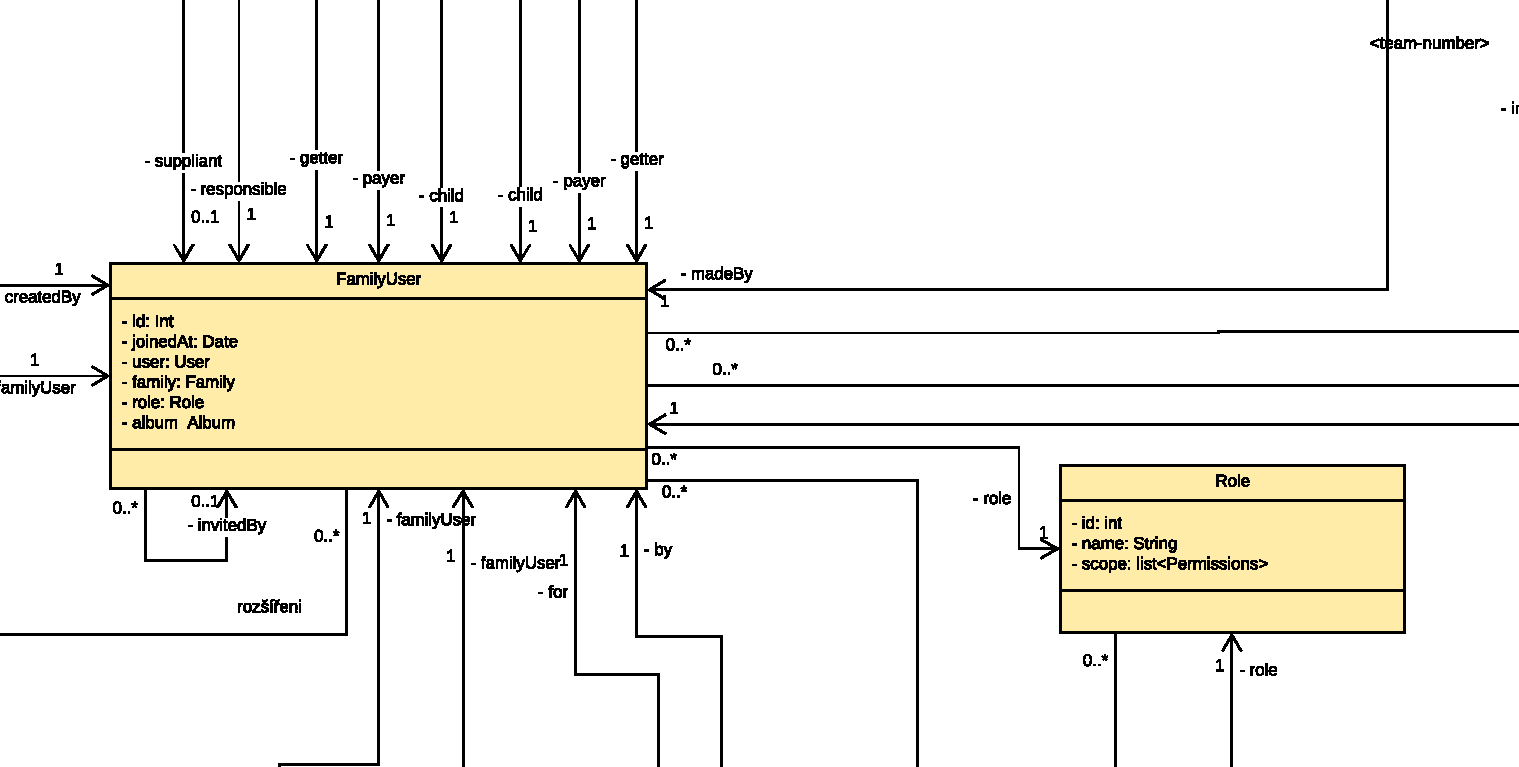
\includegraphics[width=0.7\textwidth]{pdfs/Role1}
	        \caption[Návrh Rolí]{Návrh třídy Role podle Doménovém modelu z předmětu BI-SP2}\label{image:Role1}
        \end{figure}
    
        \subsection{Autorizace}
            Bezpečnost serveru je možné rozdělit do dvou častí. 
            Návrh bezpečné aplikace nebyl cílem předmětu zmíněných v sekcích \ref{analyza:navrh:sp1} a \ref{analyza:navrh:spě}.

\chapter{Návrh}
Většina návrhu se zůstala stejnou, ale...
\section{Navržené úpravy}
    \subsection{Interval}
    \begin{figure}\centering
	    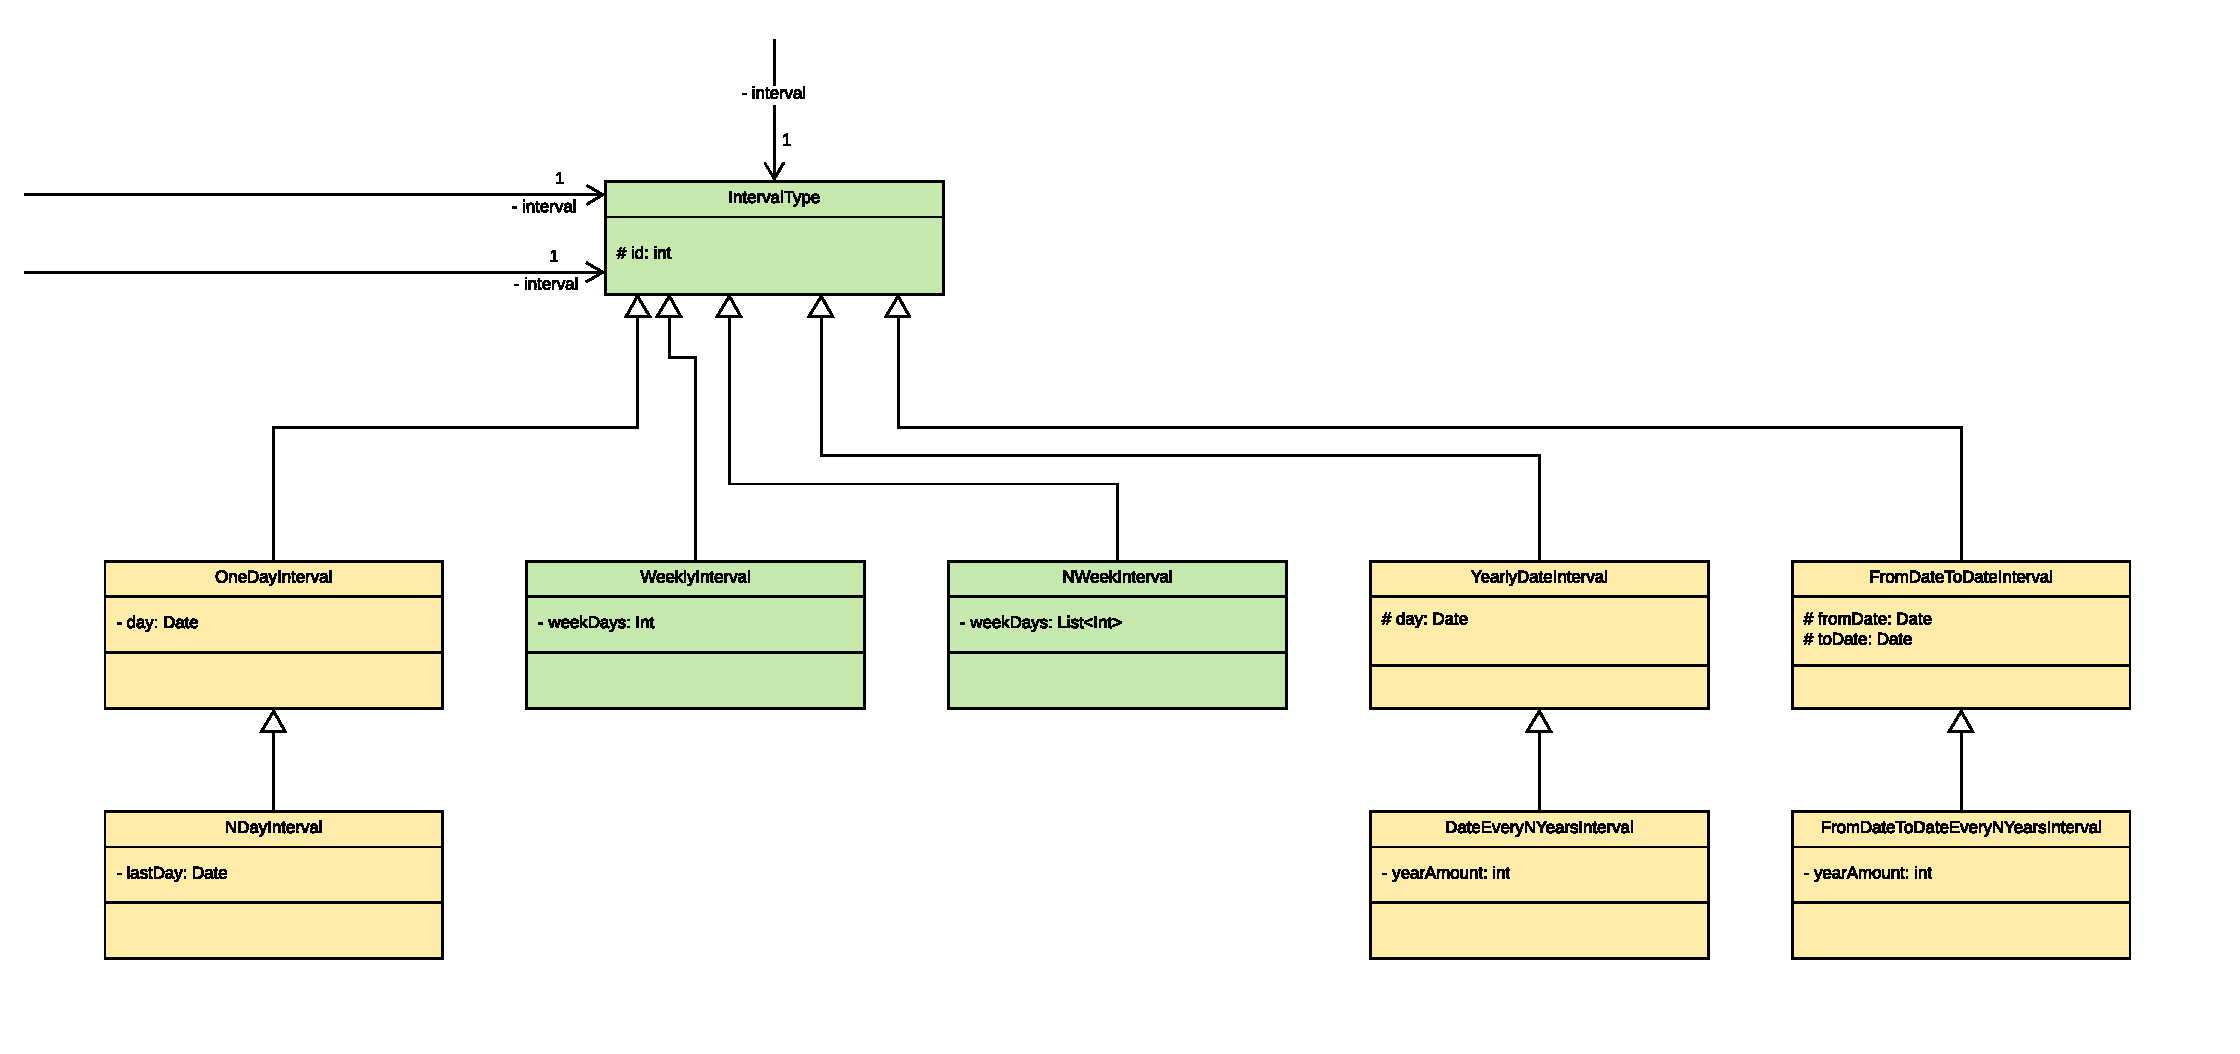
\includegraphics[width=1.0\textwidth]{pdfs/Interval1}
	    \caption[Návrh intervalu]{Návrh intervalu v Doménovém modelu z předmětu BI-SP2}\label{image:Interval1}
    \end{figure}
\section{Navržené bezpečnosti}
\section{Návrh testování}

\chapter{Implementace}

\section{Dokumentace API}
\section{Intervaly}
\section{Profily aplikace}
Aplikace má root uźivatele, který by neměl vyskytovat v produkce.
\section{Bezpečnost}

\chapter{Testování}
Nedílnou součástí vývoje softwaru je testování. Testování bylo rozděleno do dvou vrstev. Základní vrstvou jsou unit testy. Pro tvorbu těchto testů byl použit framework JUnit 5. Druhou vrstvou jsou integrační testy, které jsou implementovány pomoci funkcionality, kterou poskytuje framework Spring.

\section{Tagy}
    Během vývoje velkých projektů zpouštění testů je významným problémem pro programátory. 
    Framework JUnit 5 poskytuje možnost označovat metody a třídy pomocí tagu.
    
\section{Integrační testy}
\section{Unit testy}
\section{Pokrytí kódu testy}
    \subsection{JoCoCo}
    \cite{JoCoCo}
    \subsection{IntelliJ IDEA code coverage runner}
    \cite{IntelliJ IDEA code coverage runner}
\section{Zobrazování testů}


\input{latex_templates_20191223/tex/60_budouci_kroky}

\begin{conclusion}
	%space 1
%space 2 I hate this box on the top right corner
Projekt byl rozdělen do dvou samostatných častí, které byly vyvíjeny paralelně. První částí je Android aplikace. Druhou částí, která je předmětem této bakalářské práce, je serverový backend, poskytující RESTové služby pro Android aplikace.

Cílem této práce bylo navržení vhodných úprav a následná implementace existujícího návrhu a fragmentů implementace. Také zhodnocení použitelnosti výsledné implementace a navržení vhodných budoucích kroků pro pokračování vývoje serveru. Při implementaci byl také uvažován současný stav souběžně vyvíjené, frontendové části aplikace.

I~když se autor této práce zúčastnil předmětů, během kterých byl udělán předchozí návrh aplikace a fragmenty implementace, byla potřeba přezkoumat návrh programu za účelem vylepšení návrhu a eliminování nalezených nedostatků během implementace frontendové a backendové části. Předchozí implementace programu pokrývala jenom malou část aplikace, proto skoro celá již existující implementace byla přepsána. Byl opraven doménový model, provedeny změny použité třívrstvé architektury, rozšířené API, rozšířená dokumentace API, přidán proces registrace a přihlašování uživatele a také byla implementována bezpečnost aplikace. Při implementaci byly uvazovány požadavky kolegy, který souběžně vyvíjí frontendovou část aplikace.

% Práce se začíná analýzou existujícího návrhu a fragmentů implementace. I když jsem zúčastnil předmětů, které se zabývali těmto návrhem a implementací, potřeboval jsem přezkoumat celý návrh za účelem eliminování, nalezených během implementace frontendové a backendové častí, nedostatků a navržení lepších řešení.
% Potom jsem návrh novou verzí řešení, která obsahuje úpravy podle požadavků frontendové části aplikace a zároveň obsahuje navržené mnou úpravy. Implementace navrženého řešení byla nejsložitější častí této bakalářské práci, protože jsem neměl zkušeností ve vývoje projektů porovnatelného rozsahu a potřeboval jsem naučit mnoha novým věcem.
Důležitou částí této práce bylo testování, které je v~rozsahu napsaného kódu porovnatelné s~implementací serveru samotného. Testy byly rozděleny do dvou typů: unit testy a integrační testy. Unit testy testují samostatně testovatelné funkce programu. Integrační testy využívají za běhu celý kontext aplikace a testují, jestli jednotlivé řadiče fungují správně. 
% \begin{figure}\centering
% 	   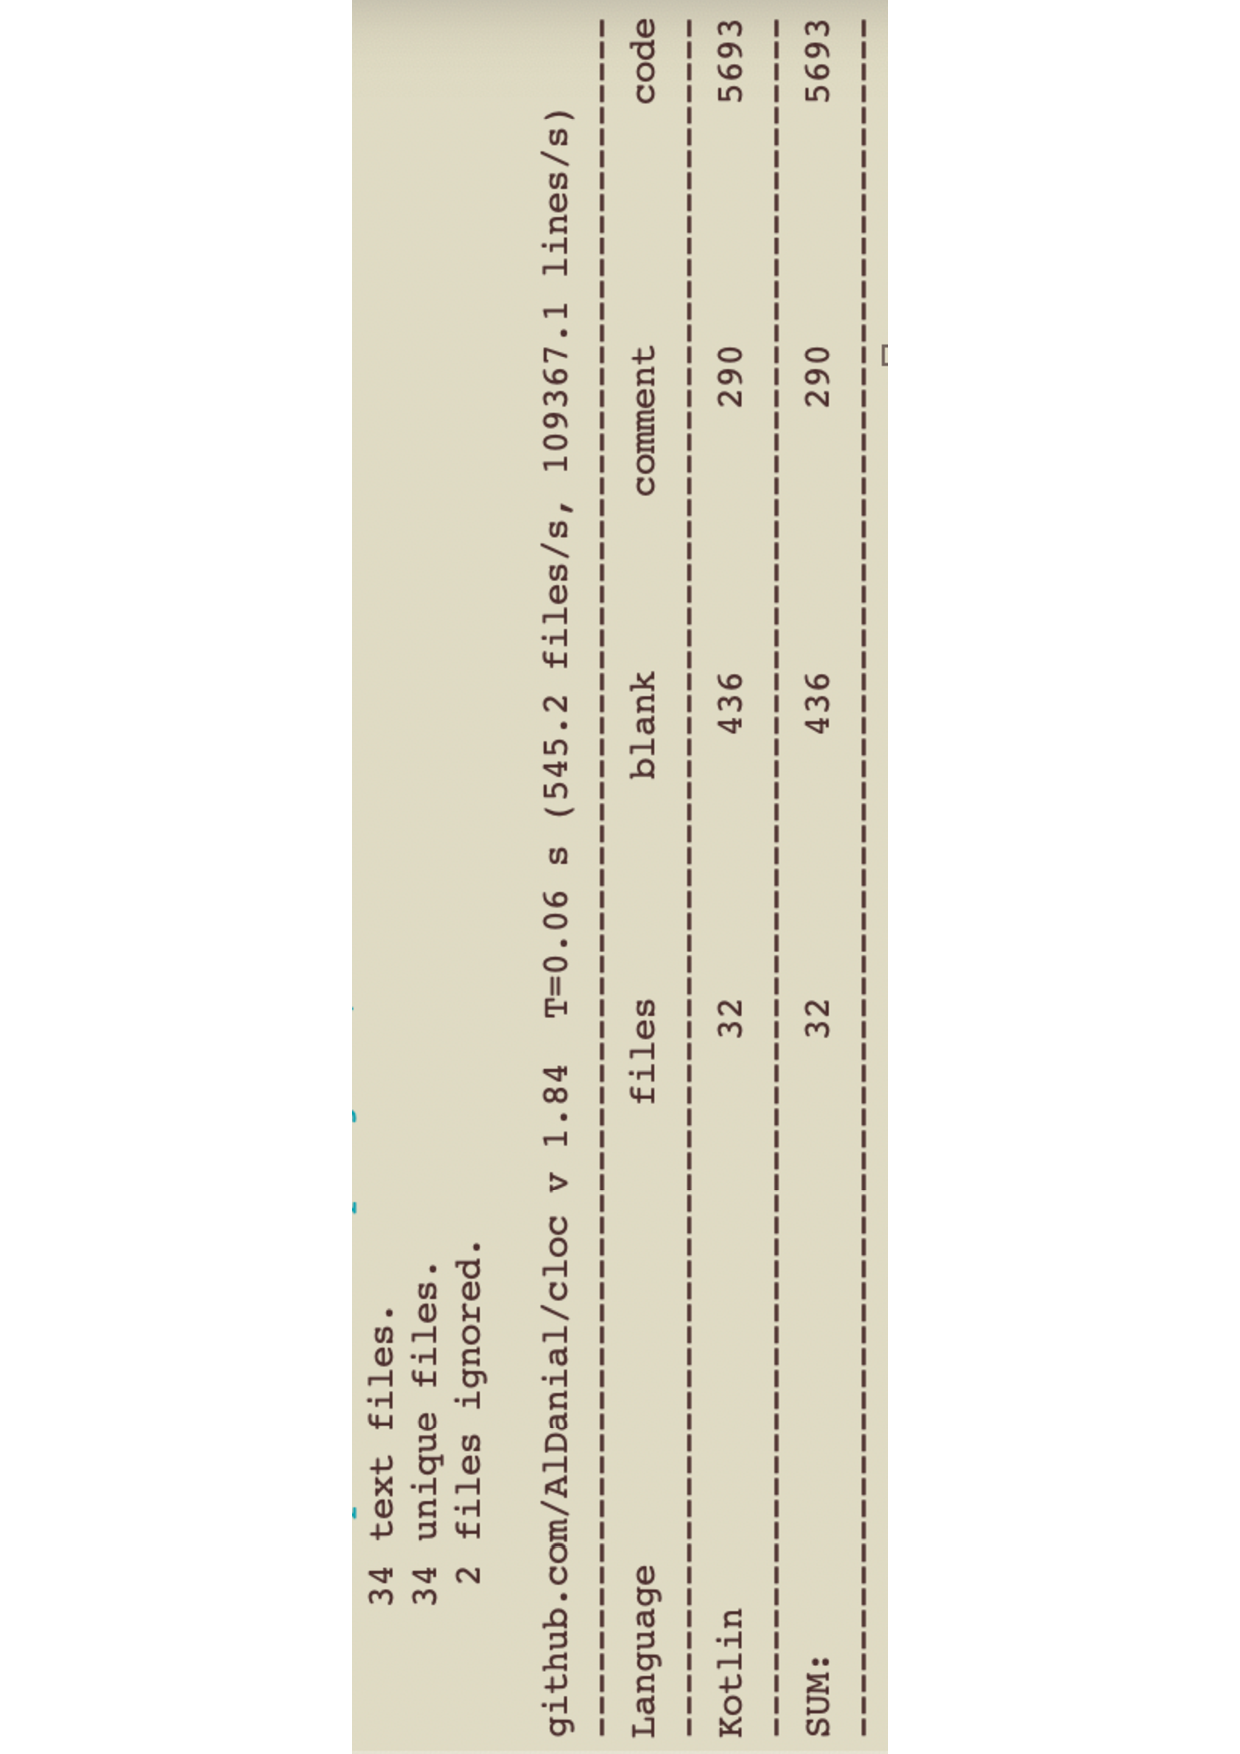
\includegraphics[angle=-90, width=0.5\textwidth]{pdfs/CodeAmountTests2}
% 	   \caption[Analýza kódu testů]{Počet napsáných řádek kódu testů}\label{image:code-count-test}
% \end{figure}
% \begin{figure}\centering
% 	   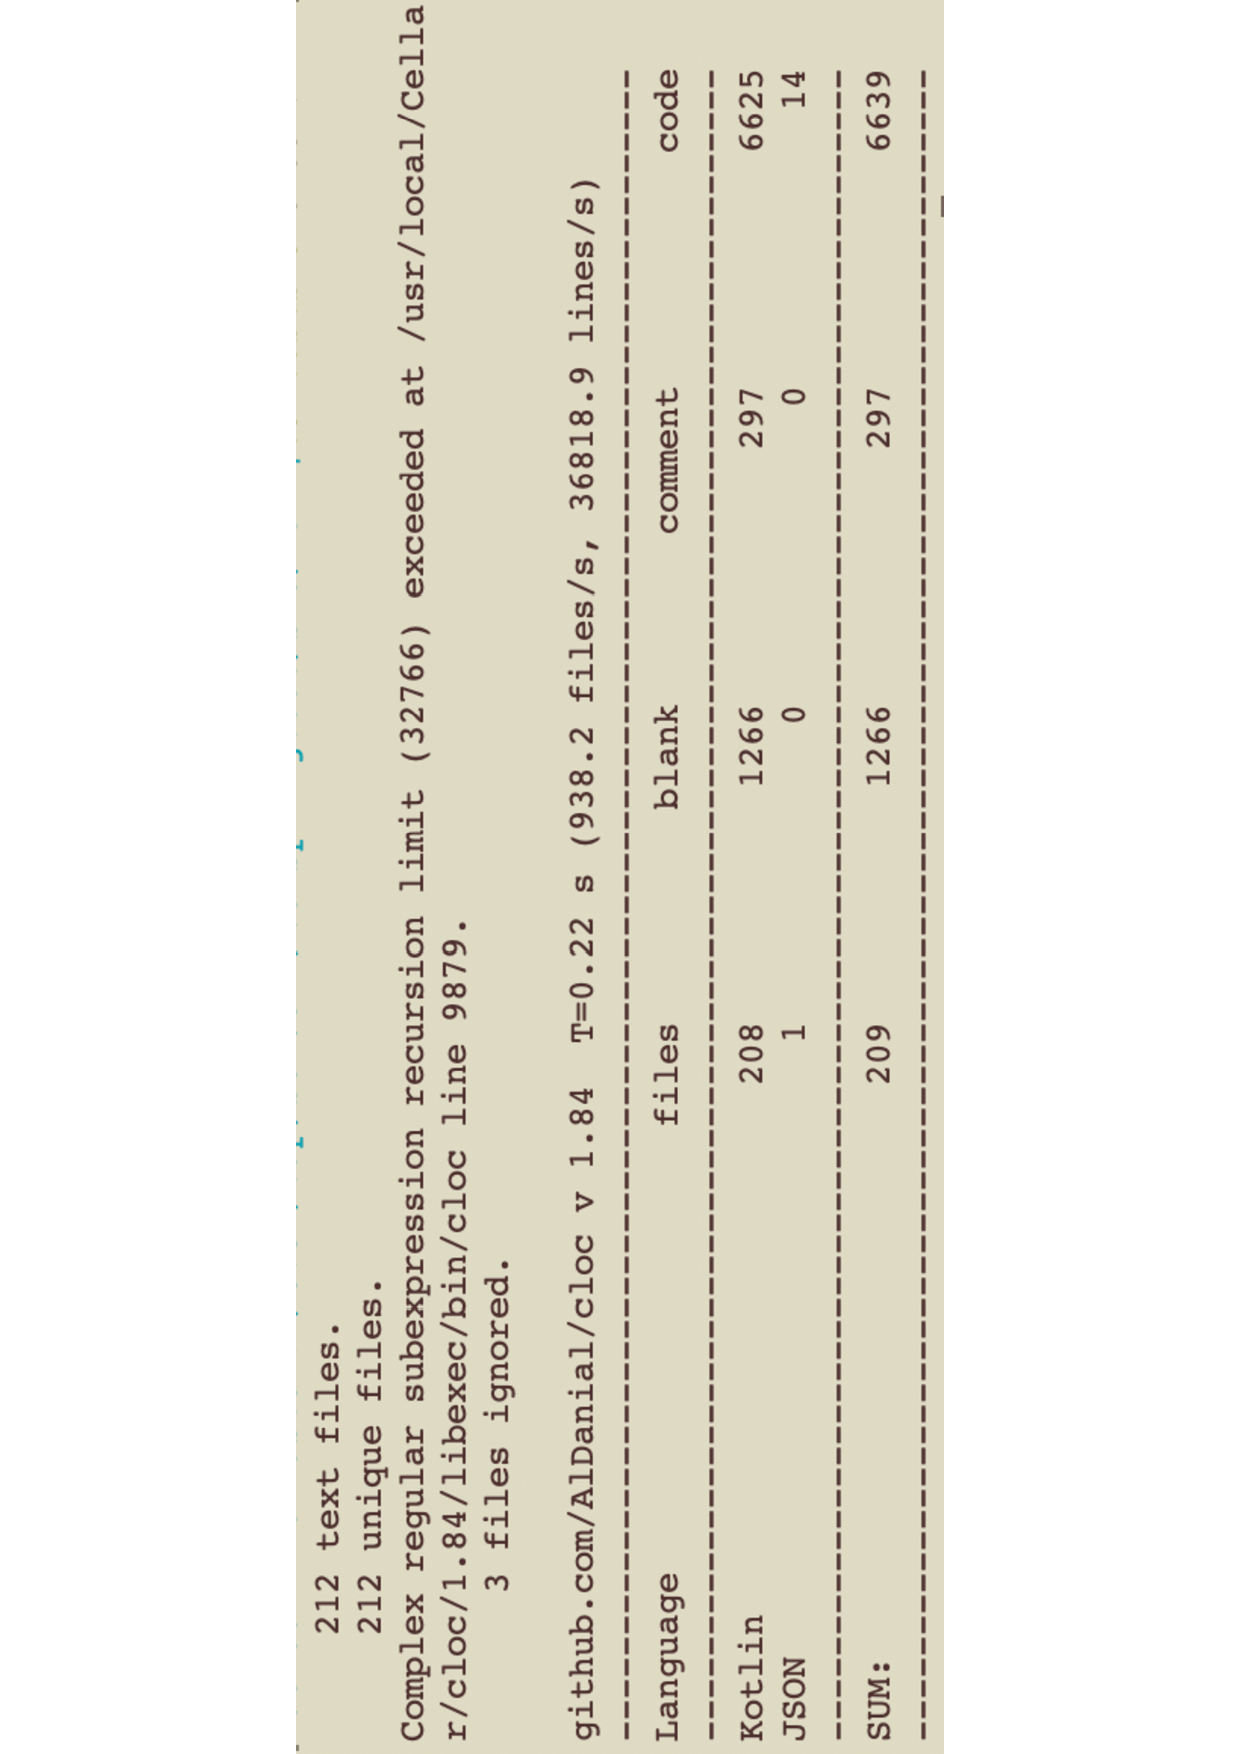
\includegraphics[angle=-90, width=0.5\textwidth]{pdfs/CodeAmountImpl2}
% 	   \caption[Analýza kódu implementace]{Počet napsáných řádek kódu za účelem implementace funkcionality}\label{image:code-count-main}
% \end{figure}

Výsledkem této bakalářské práce je funkční aplikace splňující všechny požadavky frontendové části aplikace. Ale, jak Android aplikace, tak i serverový backend ještě nejsou ve svém finálním stavu. V~rámci této práce byl zhodnocen současný stav a představeny vhodné budoucí kroky pro pokračování vývoje.
% Následující kapitola se věnuje zhodnocení použitelností výsledné implementace a navržení budoucích kroků. Výsledek ještě není připravený pro produkční prostředí a ještě ho očekává dostatečný počet vylepšení. V rámci této bakalářské práci jsem implementoval základ backendu, který má skoro celou potřebnou funkcionalitu, kromě některých věcí, které byly objevený už během pečlivého zanoření do implementace a za
% řazené do budoucích kroků.
\end{conclusion}

% \bibliographystyle{csn690}
% \bibliography{mybibliographyfile}
% \printbibliography


\printbibliography

\appendix

\chapter{Seznam použitých zkratek}
% \printglossaries
\begin{description}
	\item[GUI] Graphical user interface
	\item[XML] Extensible markup language
\end{description}

\chapter{Slovník pojmů}
\begin{description} % TODO
	\item[Backend] Část aplikace, která se stará o ukládání dat, jejich zpracování a bussiness logiku. Většinou není přímo přístupná koncovému uživateli, ten k ní přistupuje přes frontend.
\end{description}


% % % % % % % % % % % % % % % % % % % % % % % % % % % % 
% % Tuto kapitolu z výsledné práce ODSTRAŇTE.
% % % % % % % % % % % % % % % % % % % % % % % % % % % % 
% 
% \chapter{Návod k~použití této šablony}
% 
% Tento dokument slouží jako základ pro napsání závěrečné práce na Fakultě informačních technologií ČVUT v~Praze.
% 
% \section{Výběr základu}
% 
% Vyberte si šablonu podle druhu práce (bakalářská, diplomová), jazyka (čeština, angličtina) a kódování (ASCII, \mbox{UTF-8}, \mbox{ISO-8859-2} neboli latin2 a nebo \mbox{Windows-1250}). 
% 
% V~české variantě naleznete šablony v~souborech pojmenovaných ve formátu práce\_kódování.tex. Typ může být:
% \begin{description}
% 	\item[BP] bakalářská práce,
% 	\item[DP] diplomová (magisterská) práce.
% \end{description}
% Kódování, ve kterém chcete psát, může být:
% \begin{description}
% 	\item[UTF-8] kódování Unicode,
% 	\item[ISO-8859-2] latin2,
% 	\item[Windows-1250] znaková sada 1250 Windows.
% \end{description}
% V~případě nejistoty ohledně kódování doporučujeme následující postup:
% \begin{enumerate}
% 	\item Otevřete šablony pro kódování UTF-8 v~editoru prostého textu, který chcete pro psaní práce použít -- pokud můžete texty s~diakritikou normálně přečíst, použijte tuto šablonu.
% 	\item V~opačném případě postupujte dále podle toho, jaký operační systém používáte:
% 	\begin{itemize}
% 		\item v~případě Windows použijte šablonu pro kódování \mbox{Windows-1250},
% 		\item jinak zkuste použít šablonu pro kódování \mbox{ISO-8859-2}.
% 	\end{itemize}
% \end{enumerate}
% 
% 
% V~anglické variantě jsou šablony pojmenované podle typu práce, možnosti jsou:
% \begin{description}
% 	\item[bachelors] bakalářská práce,
% 	\item[masters] diplomová (magisterská) práce.
% \end{description}
% 
% \section{Použití šablony}
% 
% Šablona je určena pro zpracování systémem \LaTeXe{}. Text je možné psát v~textovém editoru jako prostý text, lze však také využít specializovaný editor pro \LaTeX{}, např. Kile.
% 
% Pro získání tisknutelného výstupu z~takto vytvořeného souboru použijte příkaz \verb|pdflatex|, kterému předáte cestu k~souboru jako parametr. Vhodný editor pro \LaTeX{} toto udělá za Vás. \verb|pdfcslatex| ani \verb|cslatex| \emph{nebudou} s~těmito šablonami fungovat.
% 
% Více informací o~použití systému \LaTeX{} najdete např. v~\cite{wikilatex}.
% 
% \subsection{Typografie}
% 
% Při psaní dodržujte typografické konvence zvoleného jazyka. České \uv{uvozovky} zapisujte použitím příkazu \verb|\uv|, kterému v~parametru předáte text, jenž má být v~uvozovkách. Anglické otevírací uvozovky se v~\LaTeX{}u zadávají jako dva zpětné apostrofy, uzavírací uvozovky jako dva apostrofy. Často chybně uváděný symbol "{} (palce) nemá s~uvozovkami nic společného.
% 
% Dále je třeba zabránit zalomení řádky mezi některými slovy, v~češtině např. za jednopísmennými předložkami a spojkami (vyjma \uv{a}). To docílíte vložením pružné nezalomitelné mezery -- znakem \texttt{\textasciitilde}. V~tomto případě to není třeba dělat ručně, lze použít program \verb|vlna|.
% 
% Více o~typografii viz \cite{kobltypo}.
% 
% \subsection{Obrázky}
% 
% Pro umožnění vkládání obrázků je vhodné použít balíček \verb|graphicx|, samotné vložení se provede příkazem \verb|\includegraphics|. Takto je možné vkládat obrázky ve formátu PDF, PNG a JPEG jestliže používáte pdf\LaTeX{} nebo ve formátu EPS jestliže používáte \LaTeX{}. Doporučujeme preferovat vektorové obrázky před rastrovými (vyjma fotografií).
% 
% \subsubsection{Získání vhodného formátu}
% 
% Pro získání vektorových formátů PDF nebo EPS z~jiných lze použít některý z~vektorových grafických editorů. Pro převod rastrového obrázku na vektorový lze použít rasterizaci, kterou mnohé editory zvládají (např. Inkscape). Pro konverze lze použít též nástroje pro dávkové zpracování běžně dodávané s~\LaTeX{}em, např. \verb|epstopdf|.
% 
% \subsubsection{Plovoucí prostředí}
% 
% Příkazem \verb|\includegraphics| lze obrázky vkládat přímo, doporučujeme však použít plovoucí prostředí, konkrétně \verb|figure|. Například obrázek \ref{fig:float} byl vložen tímto způsobem. Vůbec přitom nevadí, když je obrázek umístěn jinde, než bylo původně zamýšleno -- je tomu tak hlavně kvůli dodržení typografických konvencí. Namísto vynucování konkrétní pozice obrázku doporučujeme používat odkazování z~textu (dvojice příkazů \verb|\label| a \verb|\ref|).
% 
% \begin{figure}\centering
% 	
\includegraphics[width=0.5\textwidth, angle=30]{cvut-logo-bw}
% 	\caption[Příklad obrázku]{Ukázkový obrázek v~plovoucím prostředí}\label{fig:float}
% \end{figure}
% 
% \subsubsection{Verze obrázků}
% 
% % Gnuplot BW i barevně
% Může se hodit mít více verzí stejného obrázku, např. pro barevný či černobílý tisk a nebo pro prezentaci. S~pomocí některých nástrojů na generování grafiky je to snadné.
% 
% Máte-li například graf vytvořený v programu Gnuplot, můžete jeho černobílou variantu (viz obr. \ref{fig:gnuplot-bw}) vytvořit parametrem \verb|monochrome dashed| příkazu \verb|set term|. Barevnou variantu (viz obr. \ref{fig:gnuplot-col}) vhodnou na prezentace lze vytvořit parametrem \verb|colour solid|.
% 
% \begin{figure}\centering
% 	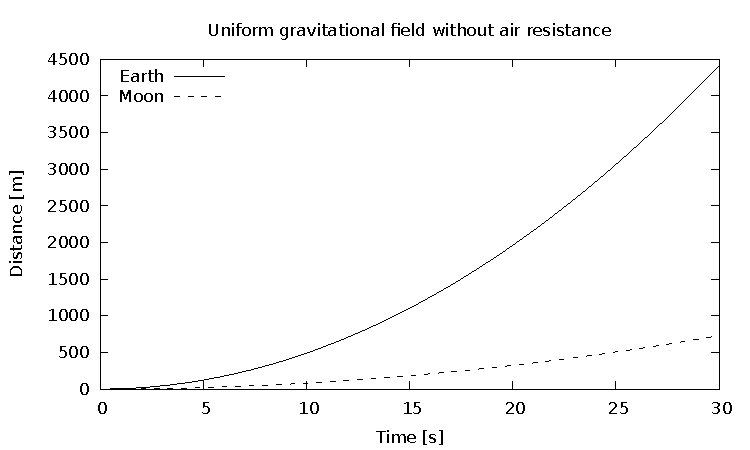
\includegraphics{gnuplot-bw}
% 	\caption{Černobílá varianta obrázku generovaného programem Gnuplot}\label{fig:gnuplot-bw}
% \end{figure}
% 
% \begin{figure}\centering
% 	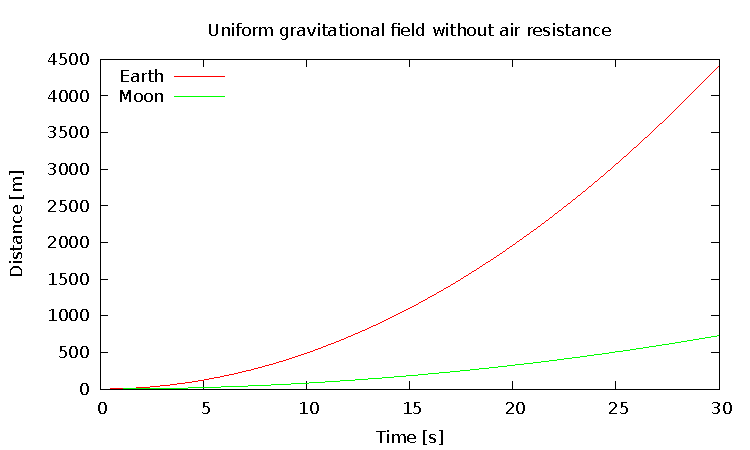
\includegraphics{gnuplot-col}
% 	\caption{Barevná varianta obrázku generovaného programem Gnuplot}\label{fig:gnuplot-col}
% \end{figure}
% 
% 
% \subsection{Tabulky}
% 
% Tabulky lze zadávat různě, např. v~prostředí \verb|tabular|, avšak pro jejich vkládání platí to samé, co pro obrázky -- použijte plovoucí prostředí, v~tomto případě \verb|table|. Například tabulka \ref{tab:matematika} byla vložena tímto způsobem.
% 
% \begin{table}\centering
% 	\caption[Příklad tabulky]{Zadávání matematiky}\label{tab:matematika}
% 	\begin{tabular}{|l|l|c|c|}\hline
% 		Typ		& Prostředí		& \LaTeX{}ovská zkratka	& \TeX{}ovská zkratka	\tabularnewline \hline \hline
% 		Text		& \verb|math|		& \verb|\(...\)|	& \verb|$...$|		\tabularnewline \hline
% 		Displayed	& \verb|displaymath|	& \verb|\[...\]|	& \verb|$$...$$|	\tabularnewline \hline
% 	\end{tabular}
% \end{table}
% 
% % % % % % % % % % % % % % % % % % % % % % % % % % % % 

% TODO uploudovat posledni verzi domenoveho modelu
\chapter{Doménový model před úpravami}\label{dodatek:DomainModel}
    \begin{figure}\centering
	    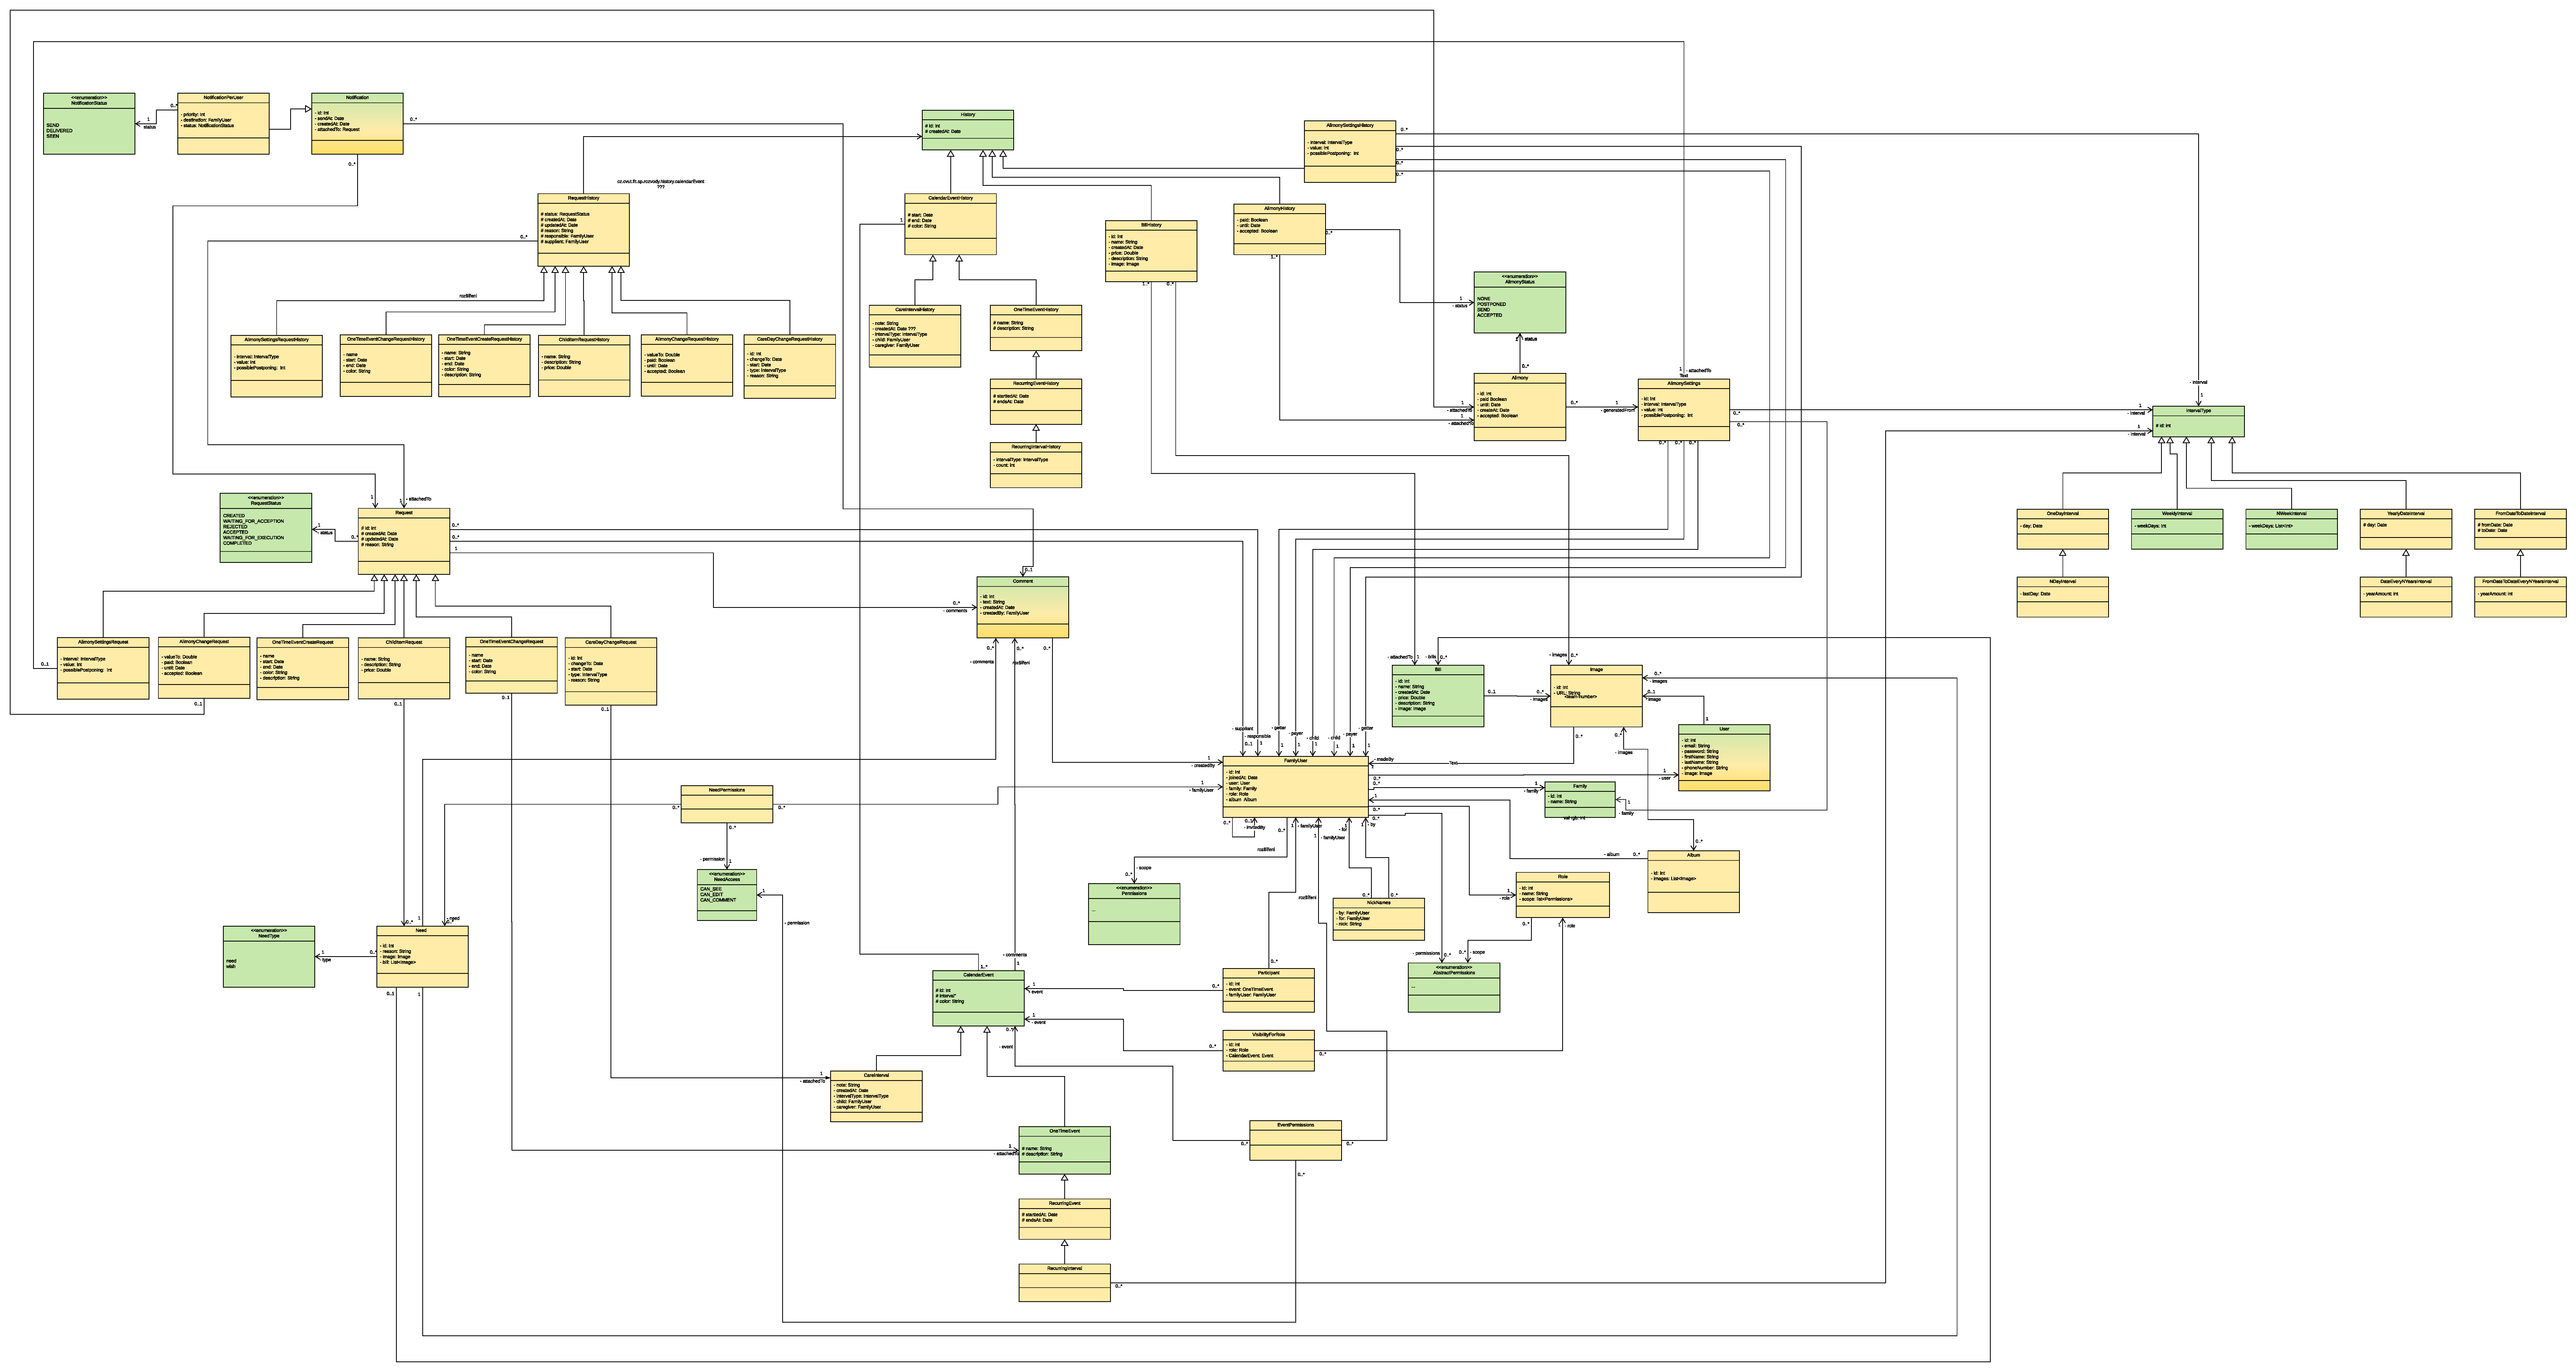
\includegraphics[angle=90, height=0.9\textheight]{pdfs/Domain-Model}
	    \caption[Doménový model před úpravami]{Doménový model z předmětu BI-SP2}\label{image:DomainModel}
    \end{figure}

\chapter{Testování}\label{dodatek:testing}
% \chapter{Pokrytí kódů testy}\label{dodatek:code-coverage}
    \begin{figure}\centering
	    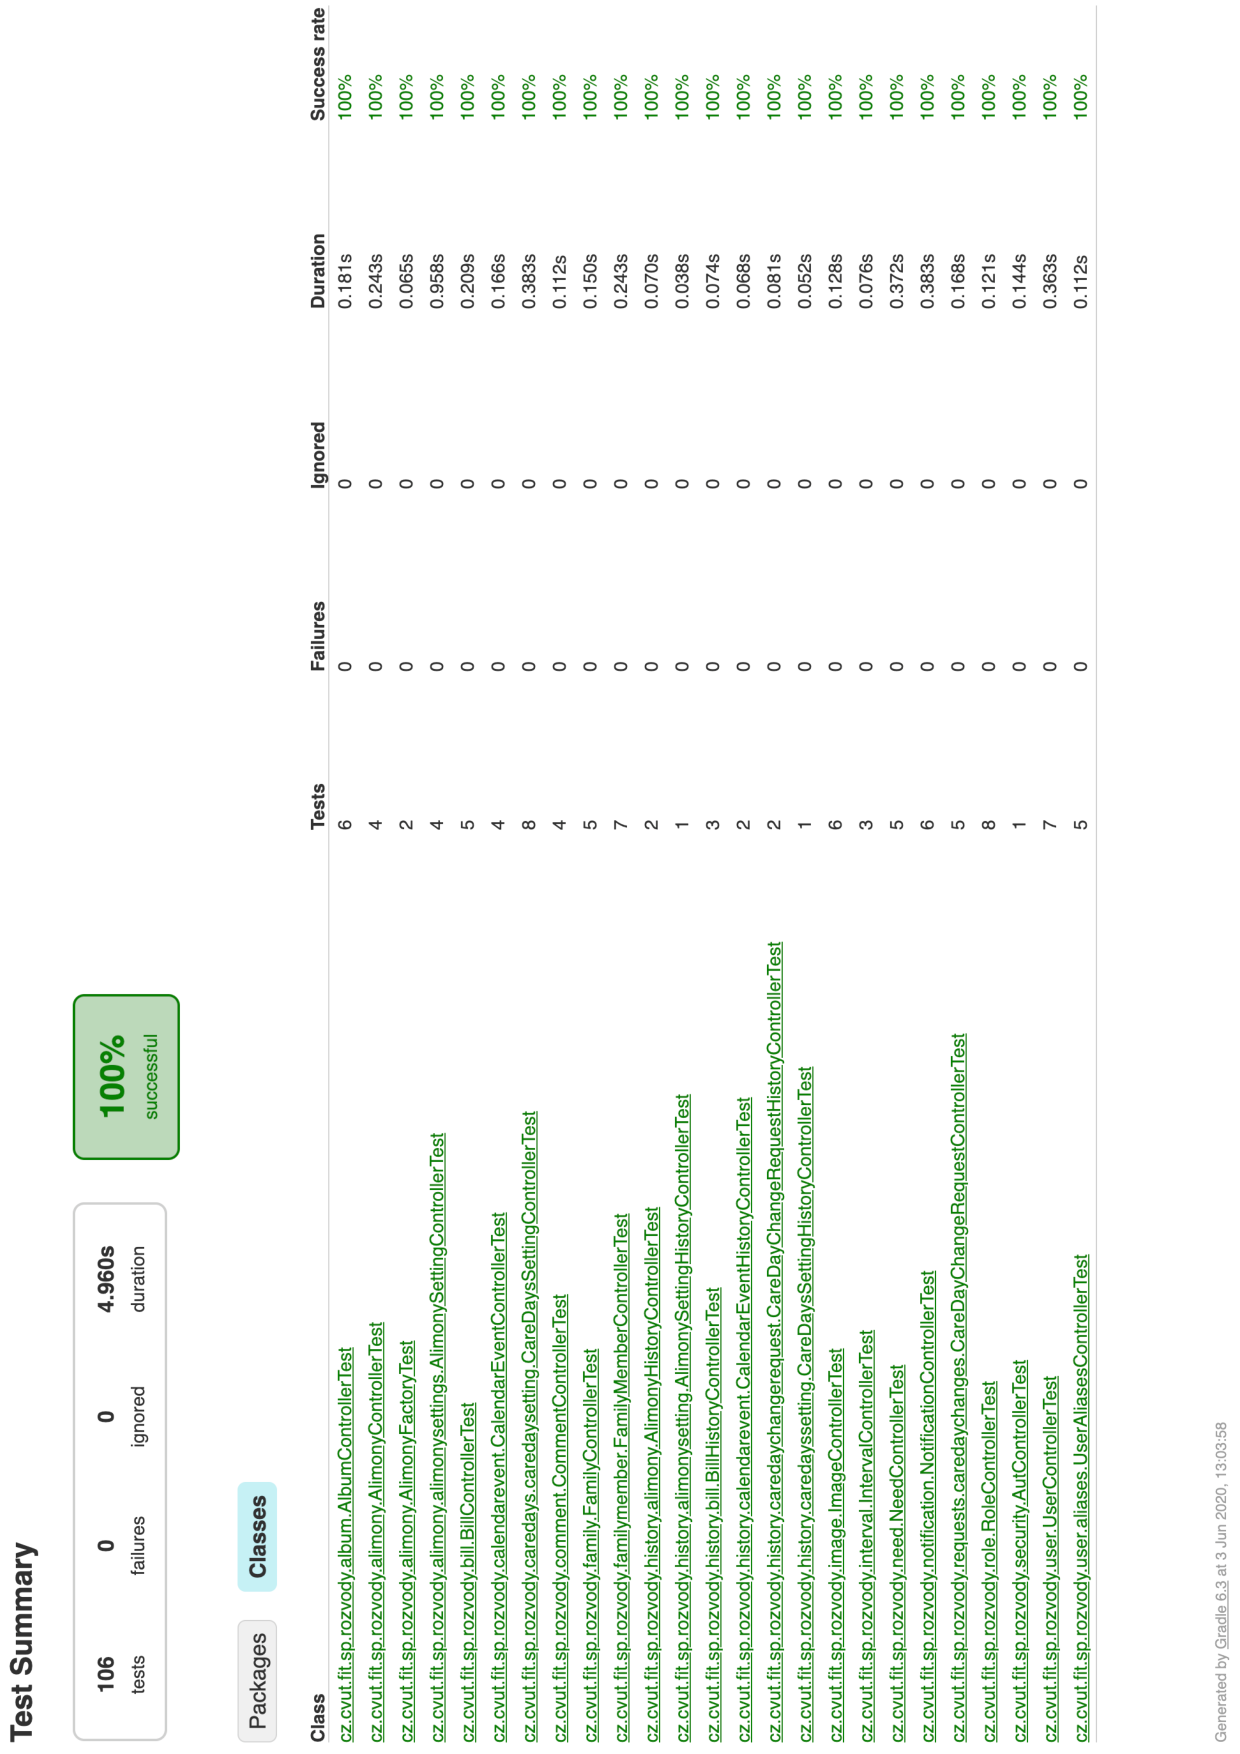
\includegraphics[width=1.0\textwidth]{pdfs/Gradle-unit-tests}
	    \caption[Seznam tříd obsahujících unit testy]{Seznam tříd obsahujících unit testy vygenerovaný pomocí nástroje Gradle}\label{image:gradle-unit-tests}
    \end{figure}
    \begin{figure}\centering
	    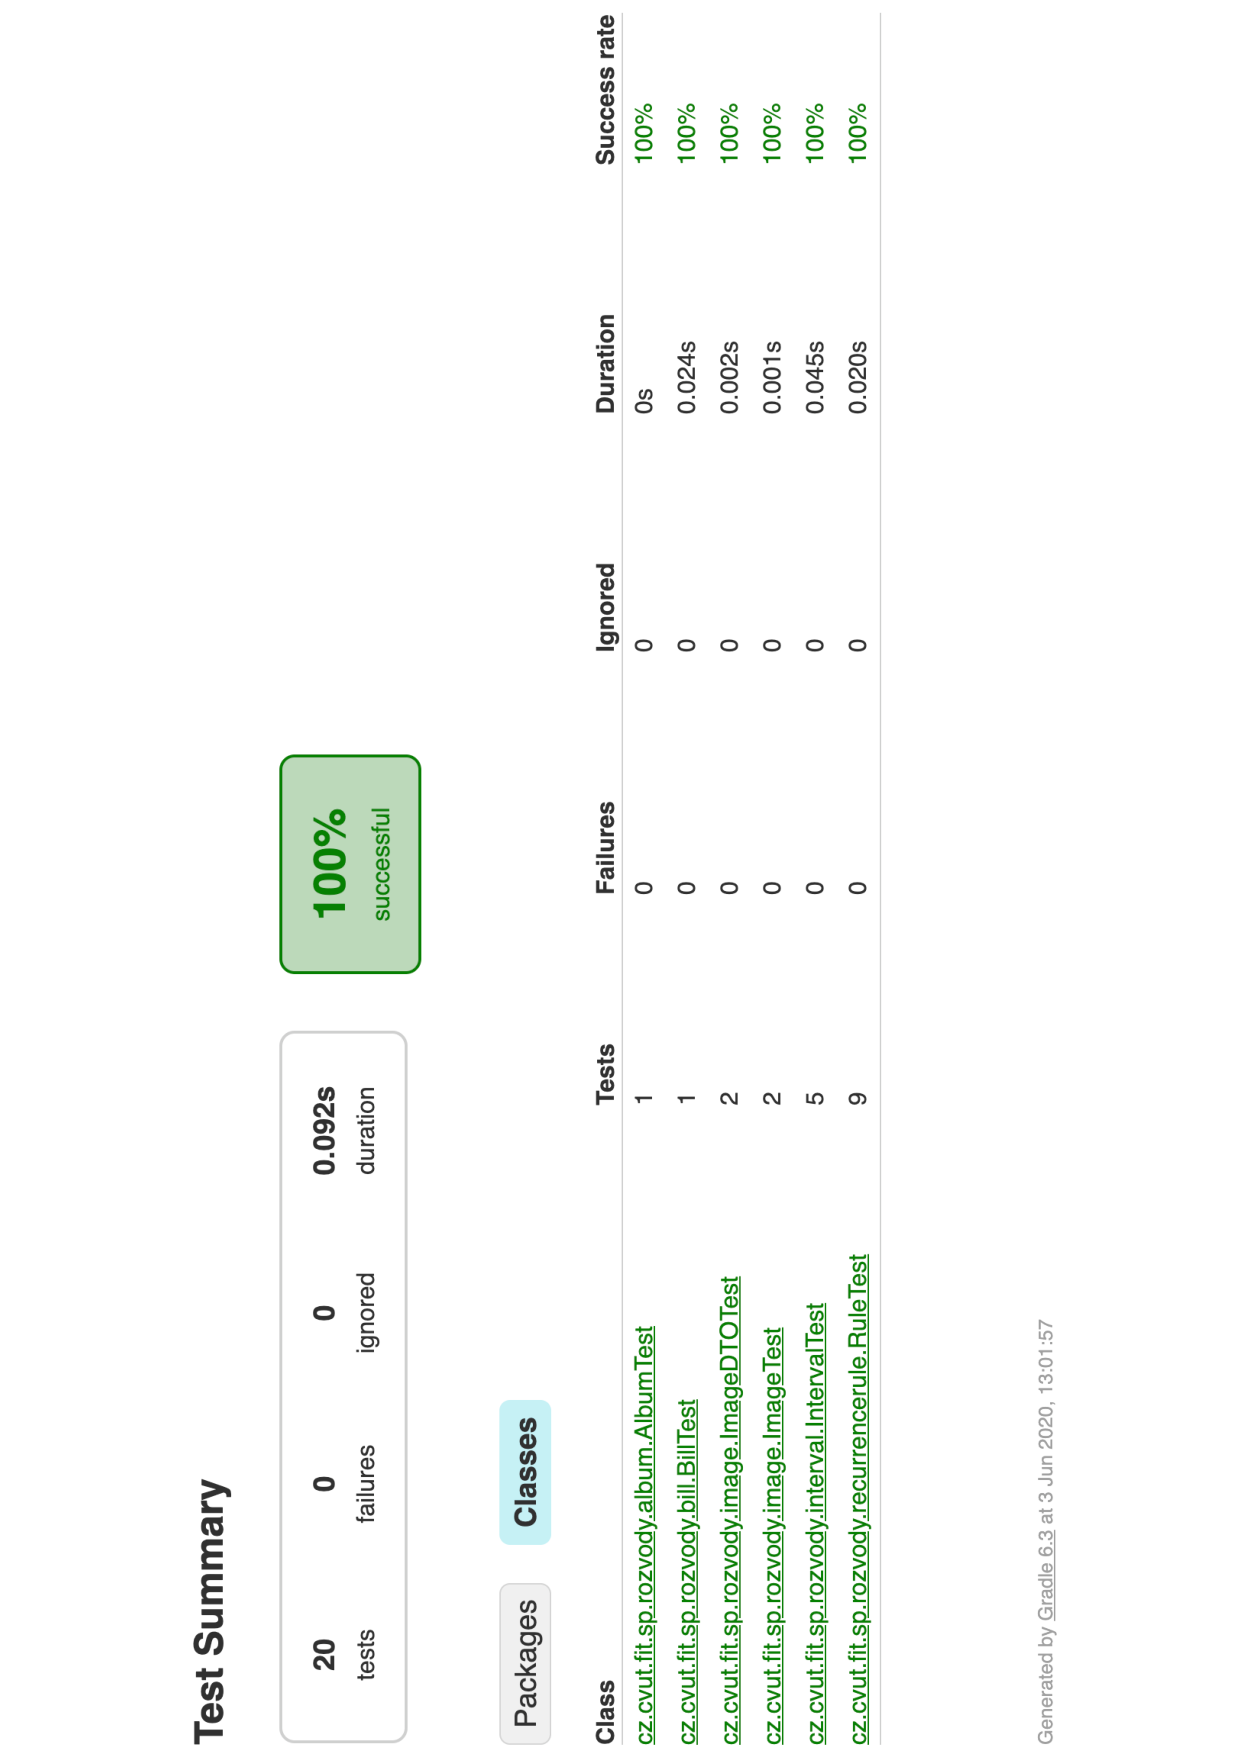
\includegraphics[width=1.0\textwidth]{pdfs/Gradle-integration-tests}
	    \caption[Seznam tříd obsahujících integrační testy]{Seznam tříd obsahující integračních testy vygenerovaný pomocí nástroje Gradle}\label{image:gradle-integration-tests}
    \end{figure}
    \begin{figure}\centering
	    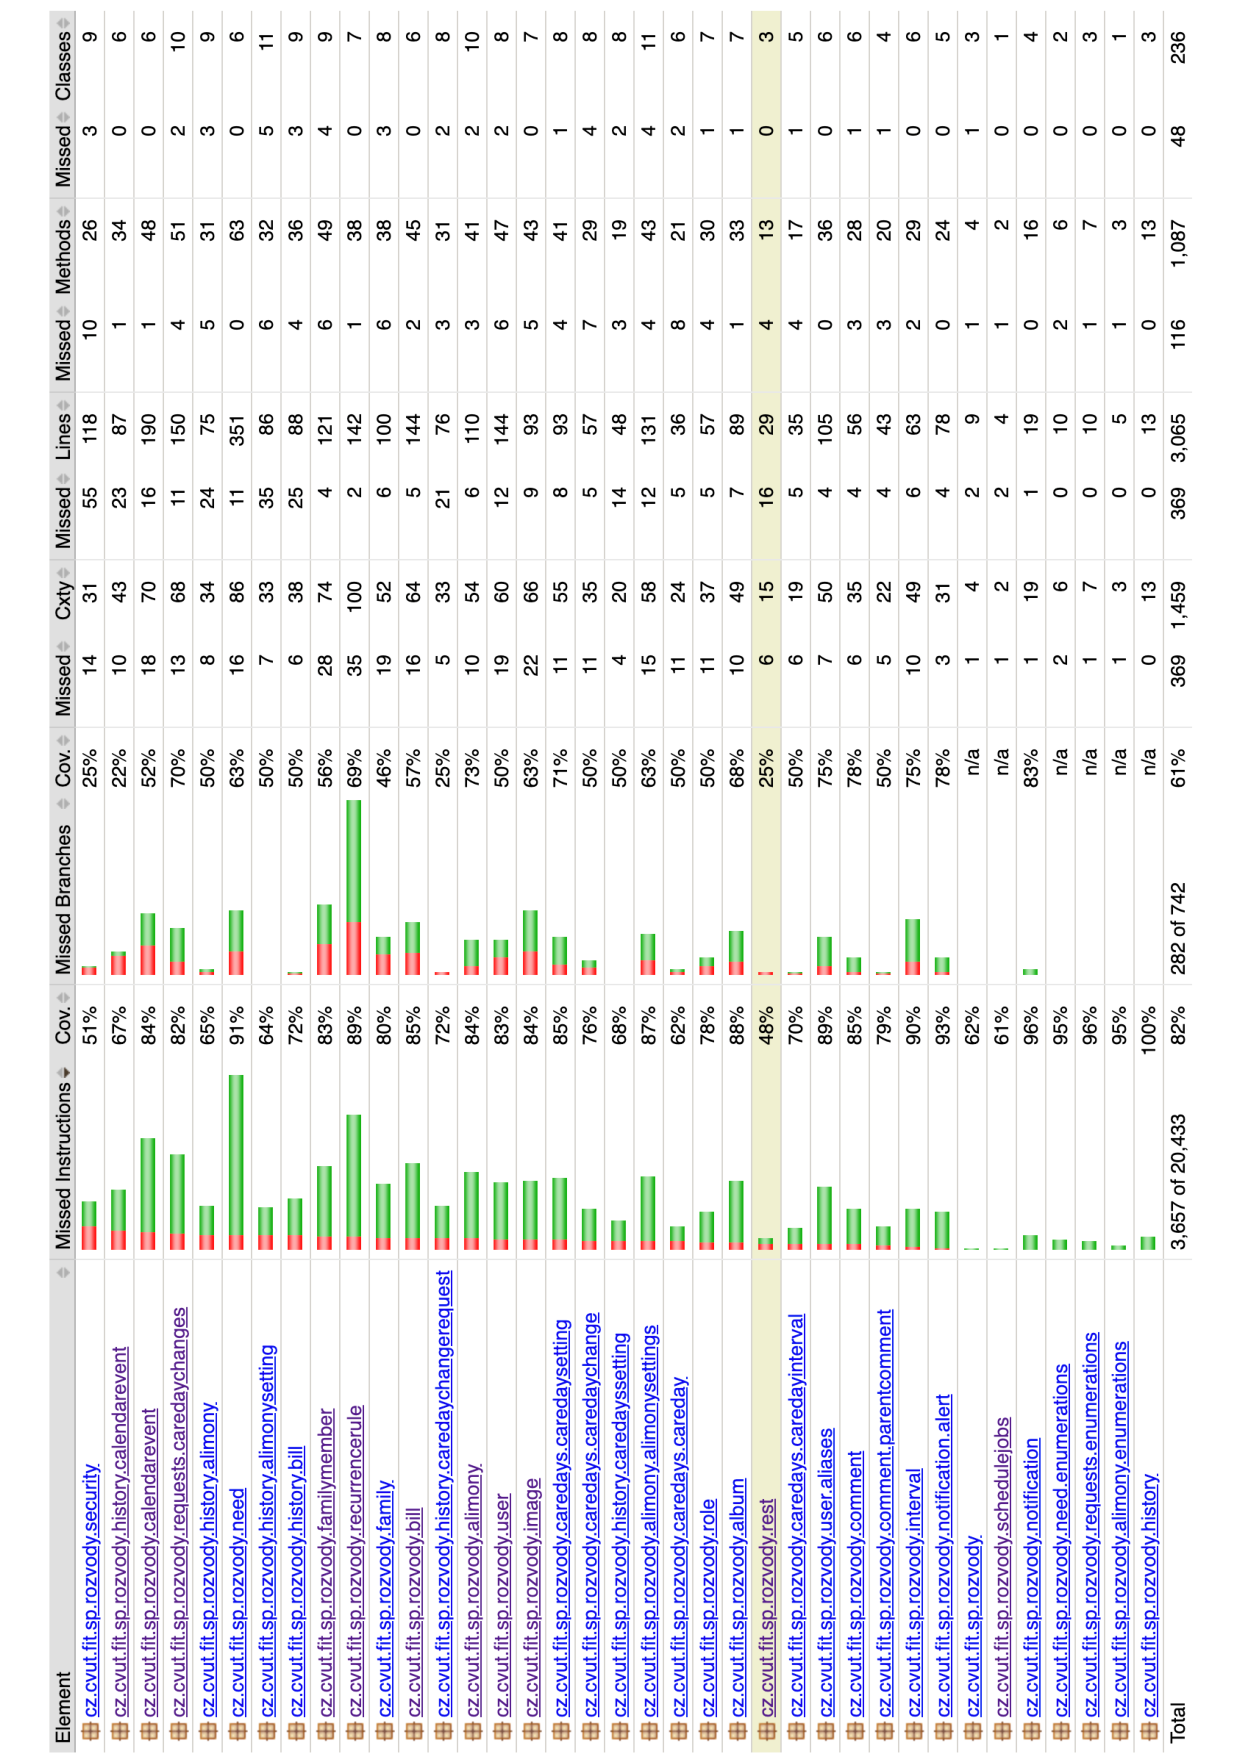
\includegraphics[width=1.0\textwidth]{pdfs/JaCoCo-results}
	    \caption[Pokrytí kódů testy podle JaCoCo]{Poslední verze výsledku pokrytí kódů testy podle JaCoCo}\label{image:jacoco-results}
    \end{figure}
    \begin{figure}\centering
	    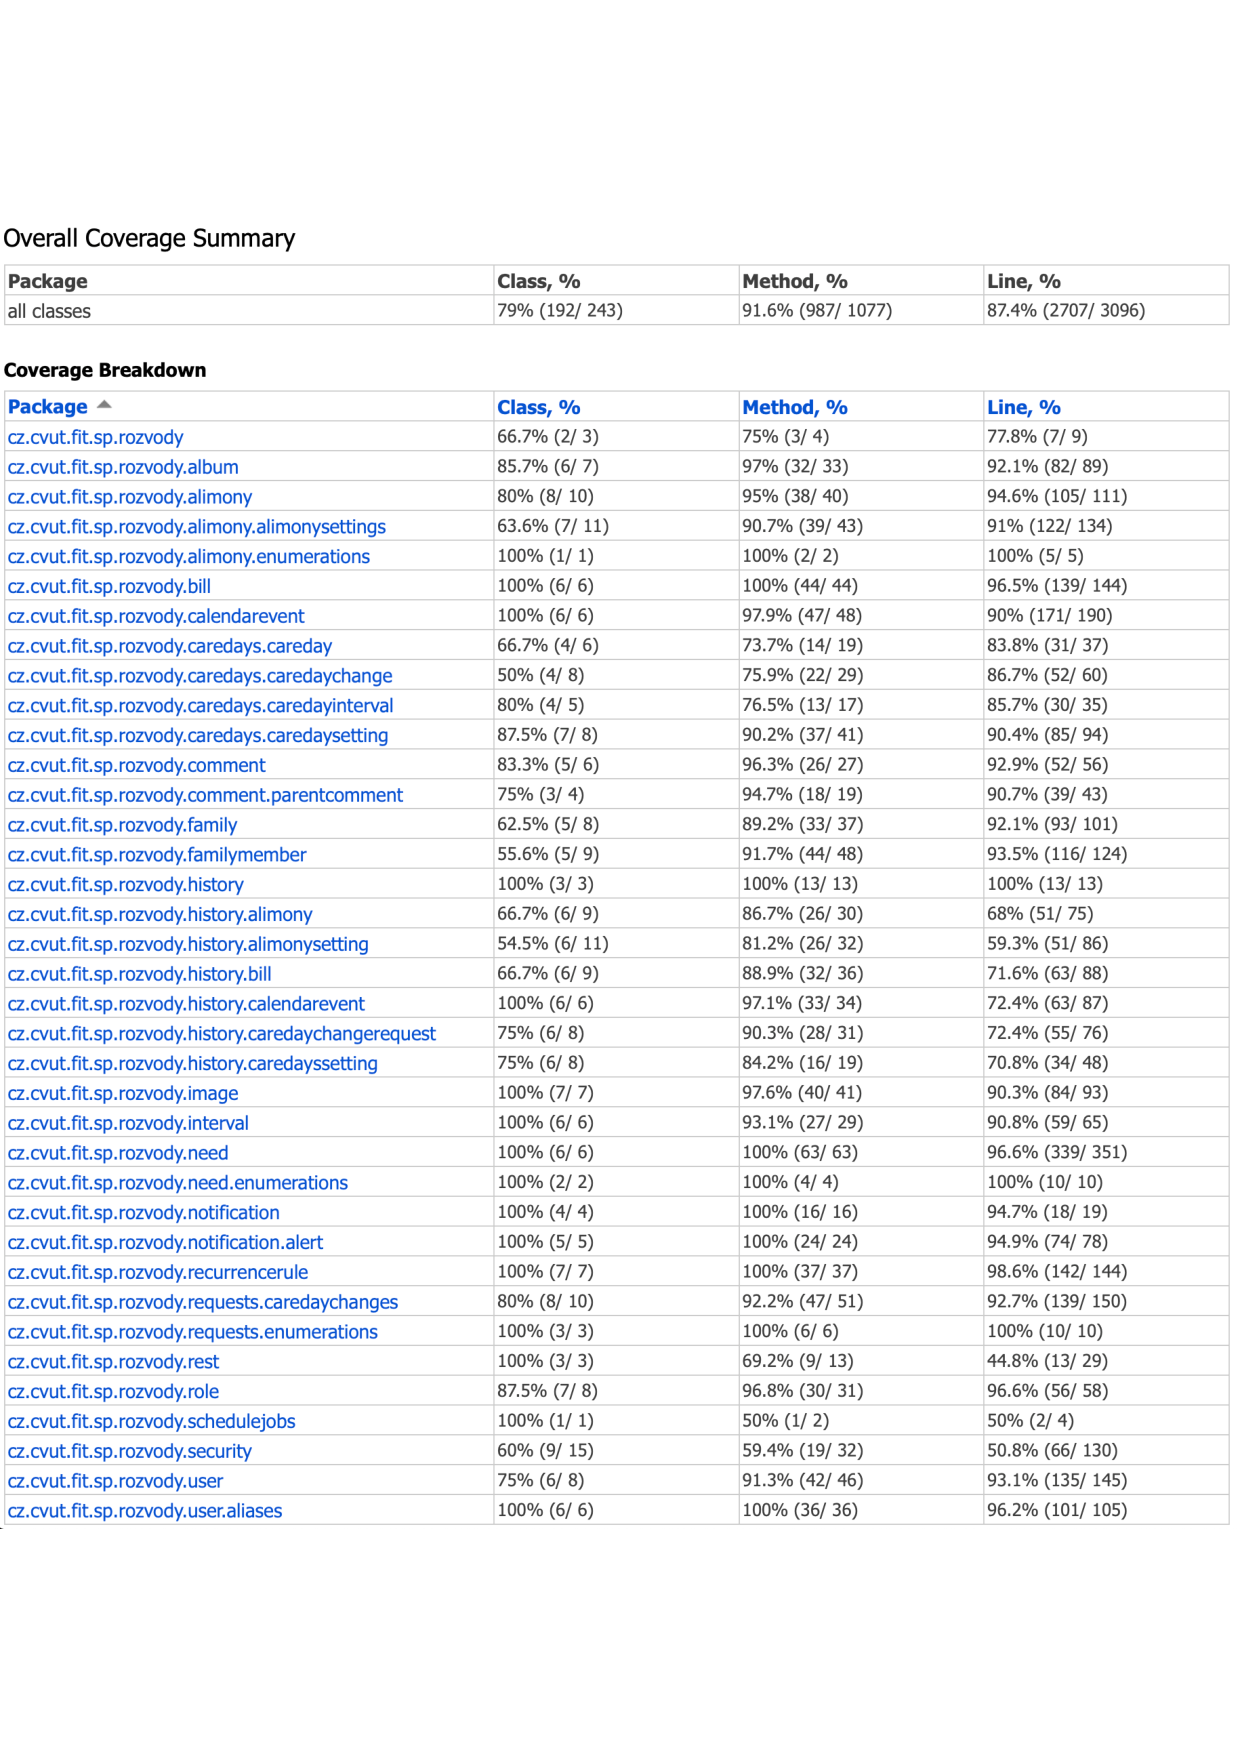
\includegraphics[width=1.0\textwidth]{pdfs/IntelliJ-IDEA-coverage-runner-results}
	    \caption[Pokrytí kódů testy podle JaCoCo]{Poslední verze výsledku pokrytí kódů testy podle IntelliJ IDEA}\label{image:intellij-coverage-result}
    \end{figure}
% TODO tady by měl být výsledný Domenový model
\chapter{Výsledný doménový model}\label{dodatek:DomainModel2}
    \begin{figure}\centering
	    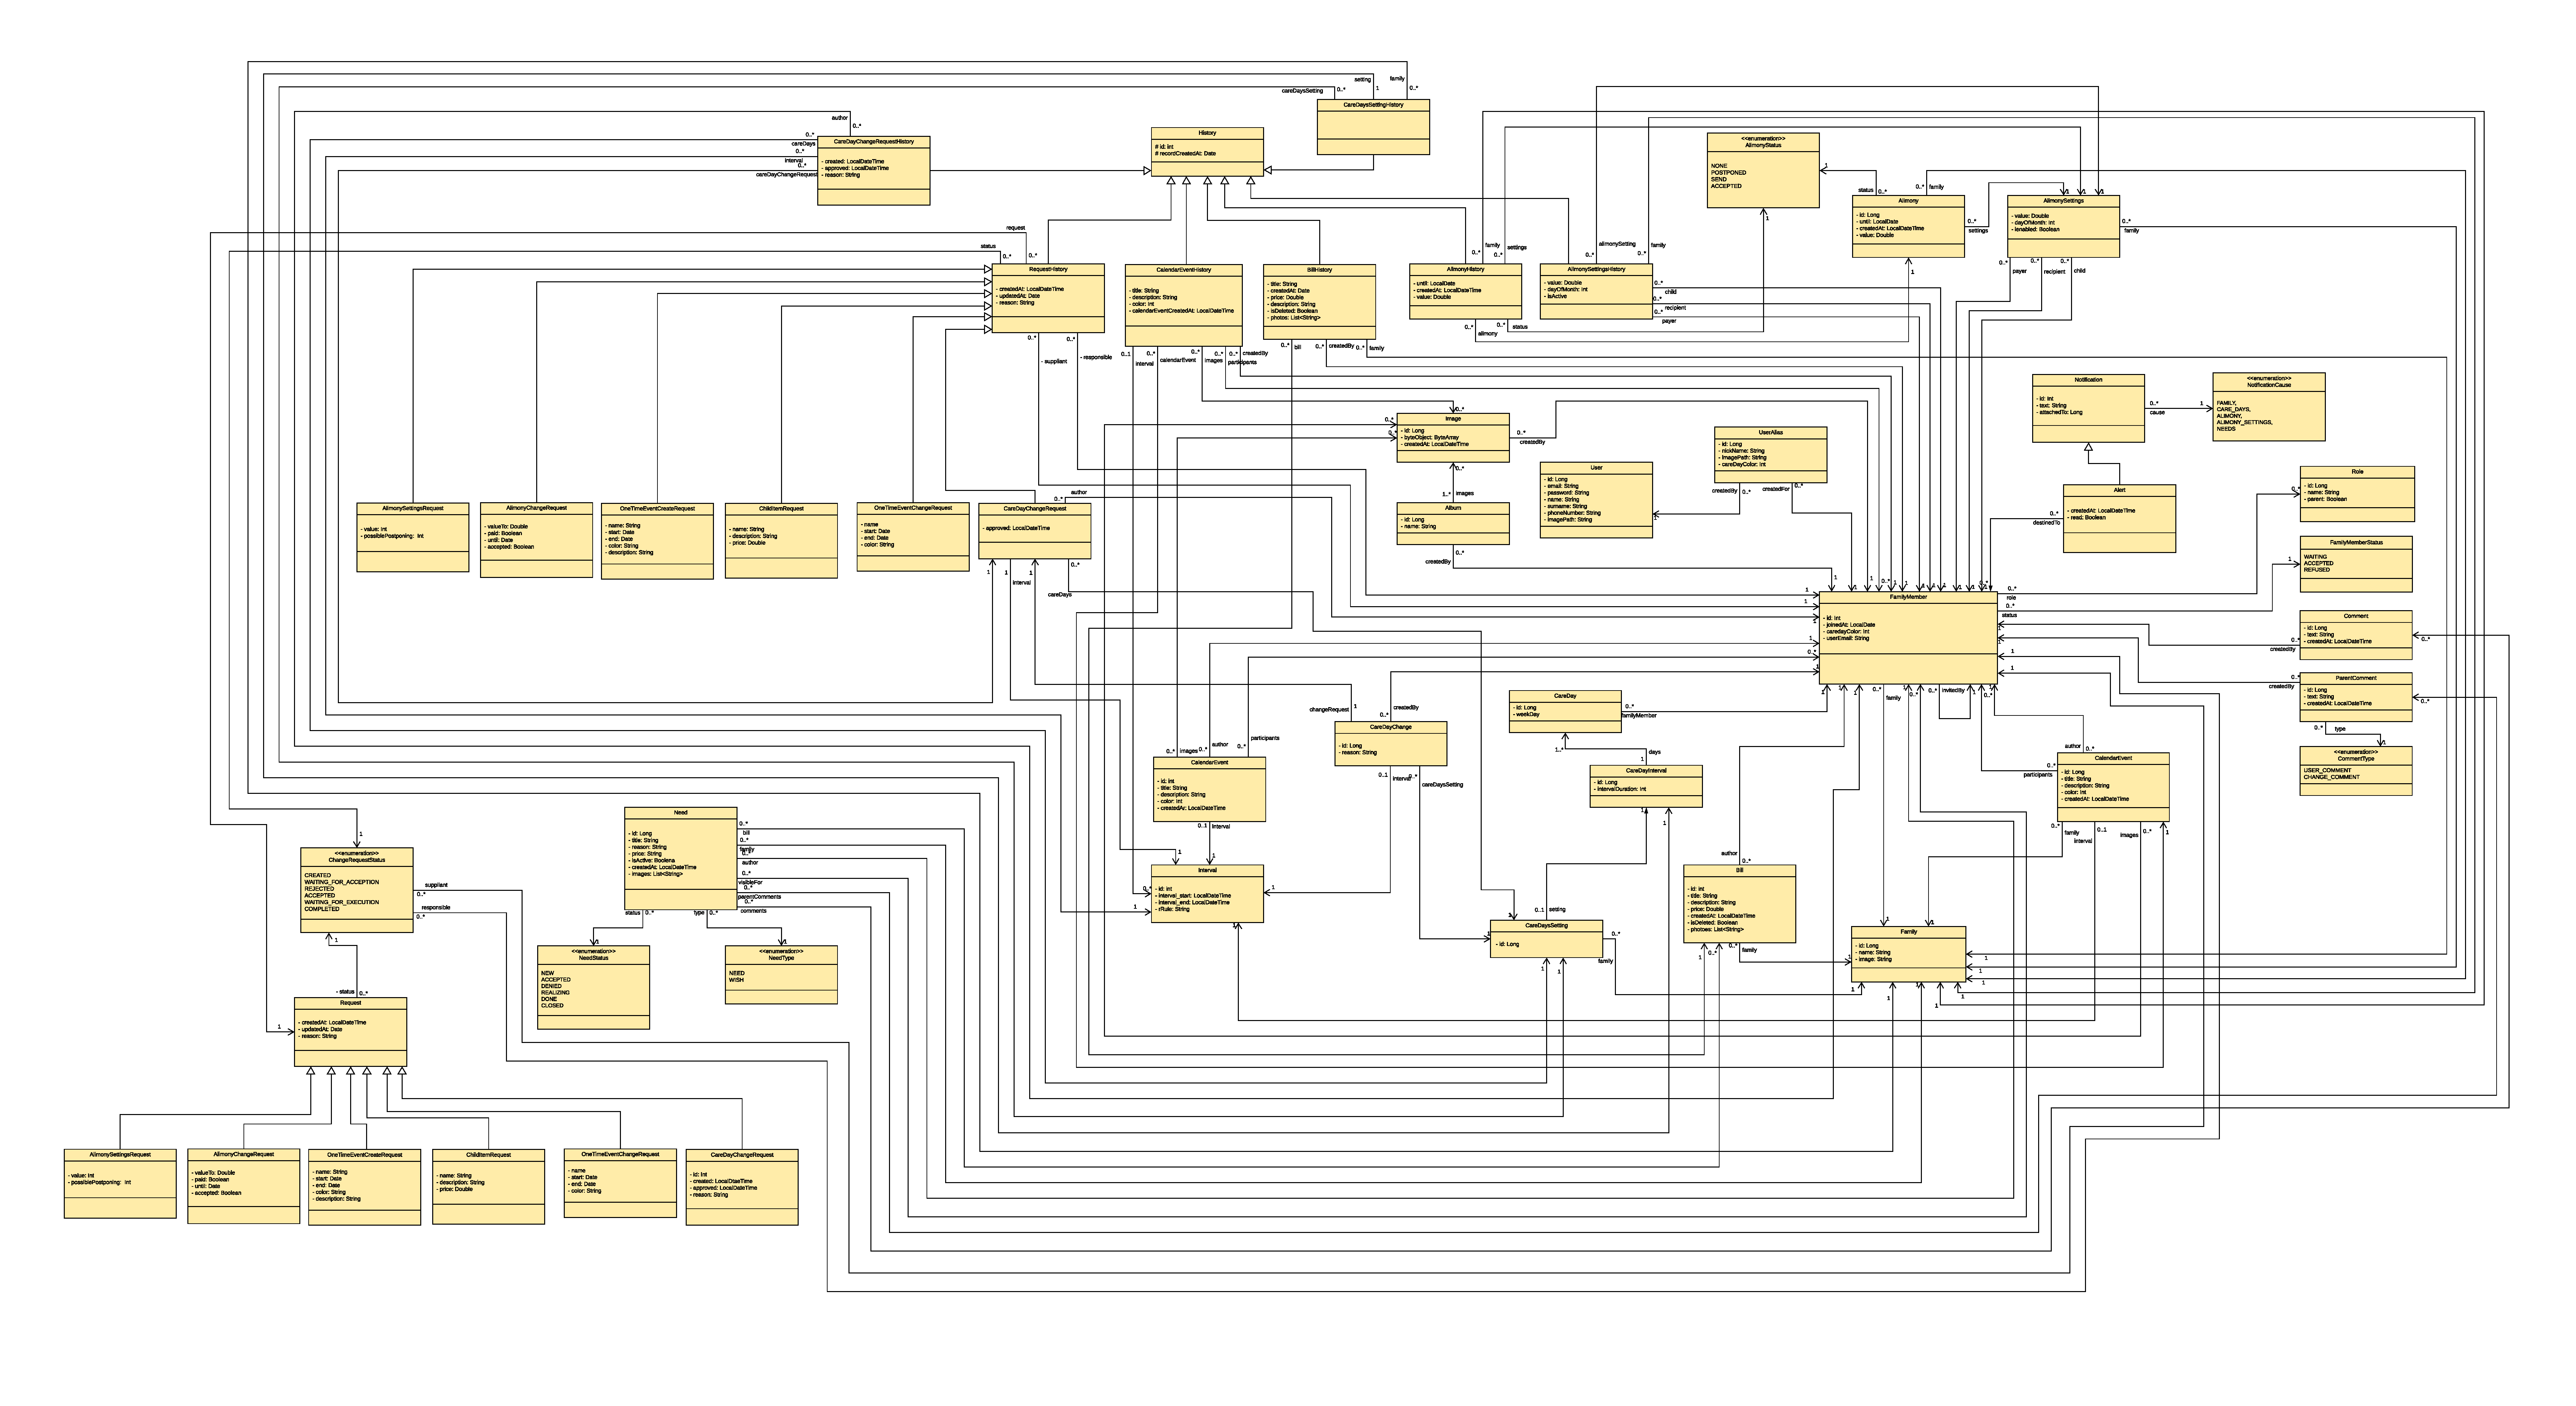
\includegraphics[angle=90, height=0.9\textheight]{pdfs/DomainModel2}
	    \caption[Výsledný doménový model]{Doménový model po navržení a implementaci všech úprav}\label{image:DomainModel2}
    \end{figure}
\chapter{Konfigurace výsledného našeptávače pro chyby}\label{dodatek:excpetion-handler2}
    % \begin{sidewaystable} \centering
    \begin{figure} \centering

    \begin{adjustbox}{angle=90} \centering
            \begin{tabular}{|l|c|c|c|}\hline
        	  Typ chyby		& HTTP status		& zpáva	& URL 	\tabularnewline \hline \hline
        	  \texttt{IllegalAccessException}	& 401	& původní zpráva chyby		& původní cesta     \tabularnewline \hline
        	  \texttt{IllegalArgumentException}	& 400	& původní zpráva chyby		& původní cesta     \tabularnewline \hline
        	  \texttt{NullPointerException}	& 500	& nic		& původní cesta     \tabularnewline \hline
        	  \texttt{No Such Element}	& 404	& nic		& nic     \tabularnewline \hline
        	  \texttt{MissingKotlinParameterException}	& 400	& původní zpráva chyby		& původní cesta     \tabularnewline \hline
            \end{tabular}
    % \end{sidewaystable}
    \end{adjustbox} \caption[Konfigurace výsledného našeptávače pro řadiče]{Ukázka výsledné konfigurace našeptávače zachycování výjimek pro řadiče}
    \end{figure}
\chapter{Obrázky}\label{dodatek:images}
    % ANALYZA
    \begin{figure}\centering
        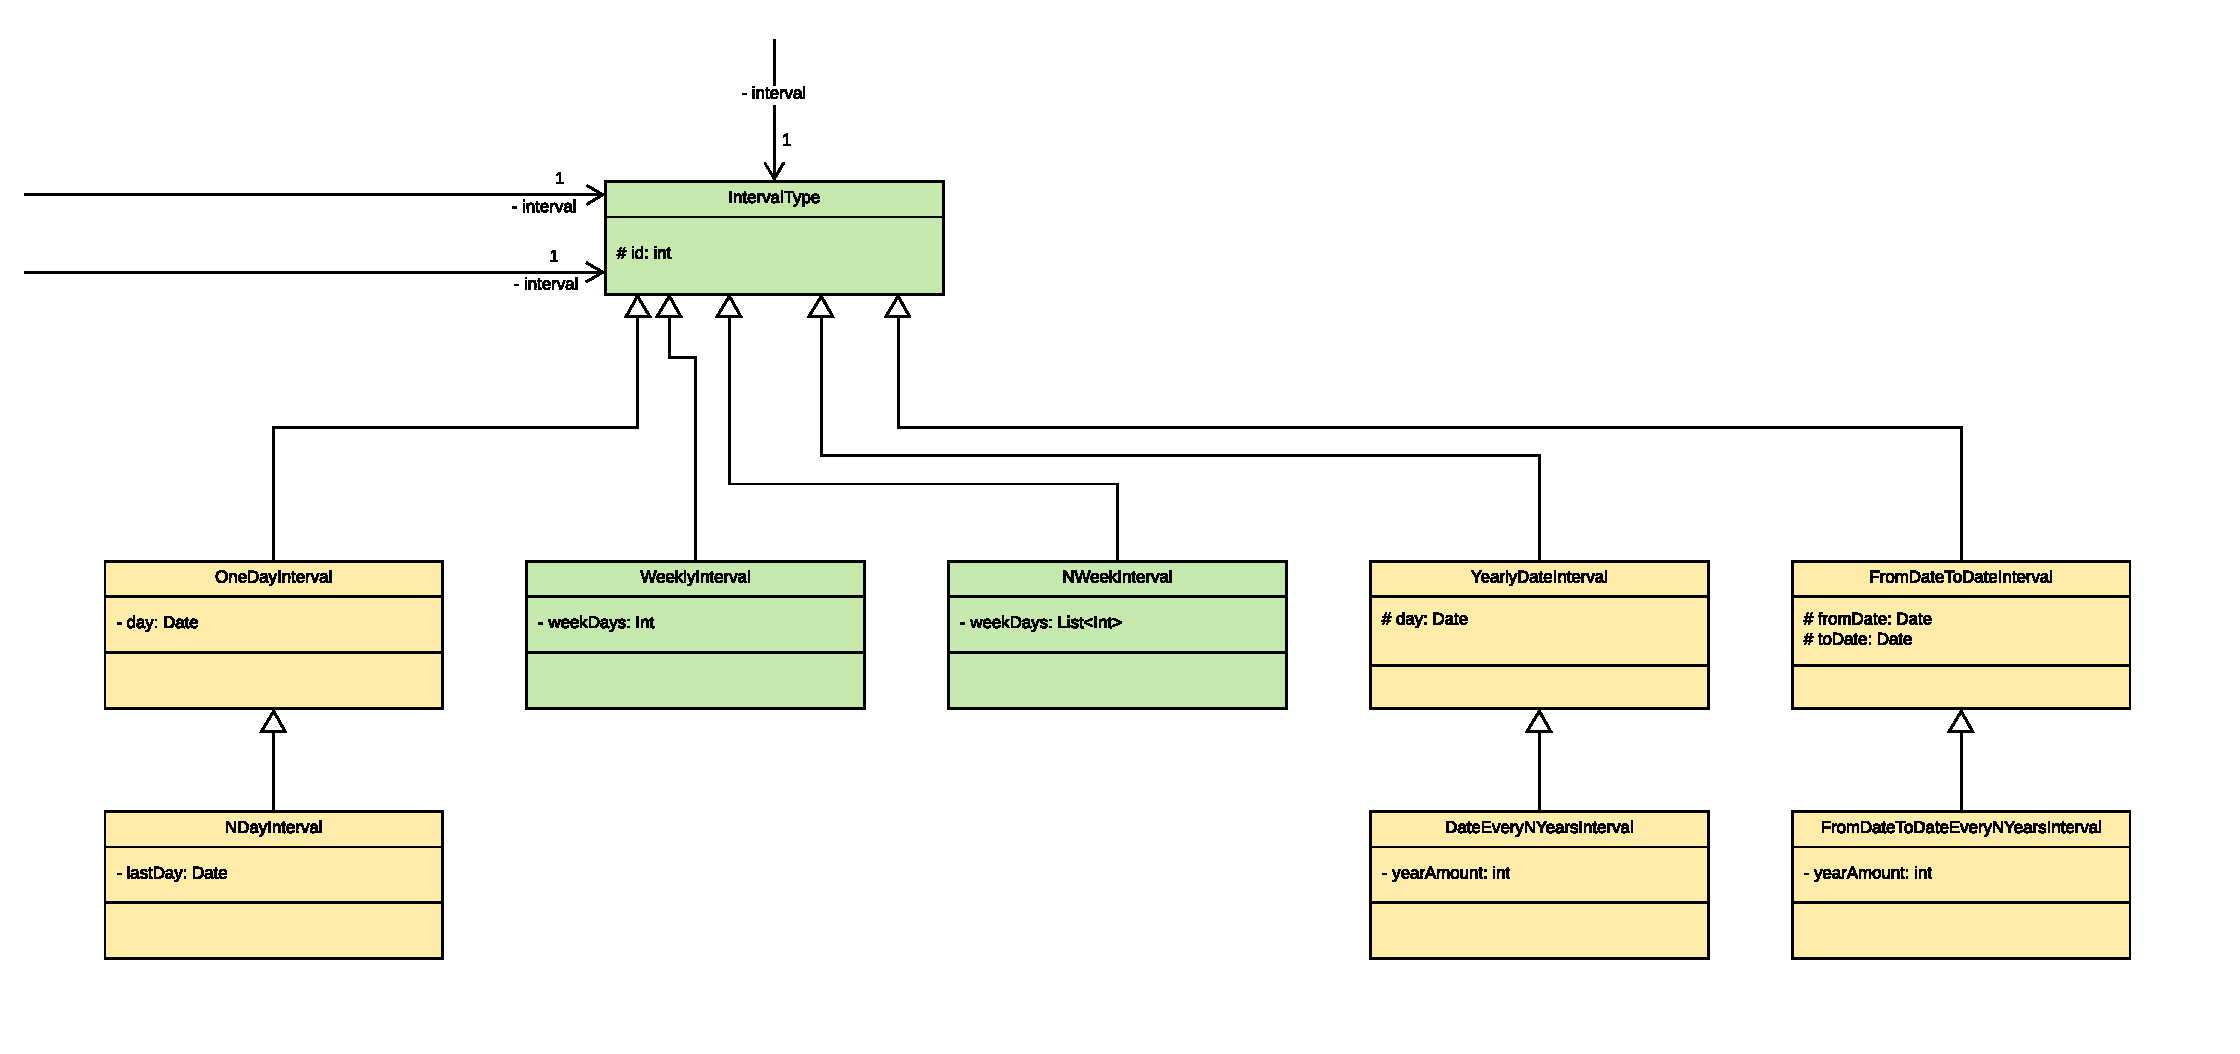
\includegraphics[angle=90, height=0.9\textheight]{pdfs/Interval1}
        \caption[Předešlý návrh entity \texttt{Interval}]{Návrh entity \textit{Interval} podle doménového modelu z předmětu BI-SP2}\label{image:Interval1}
    \end{figure}
    \begin{figure}\centering
            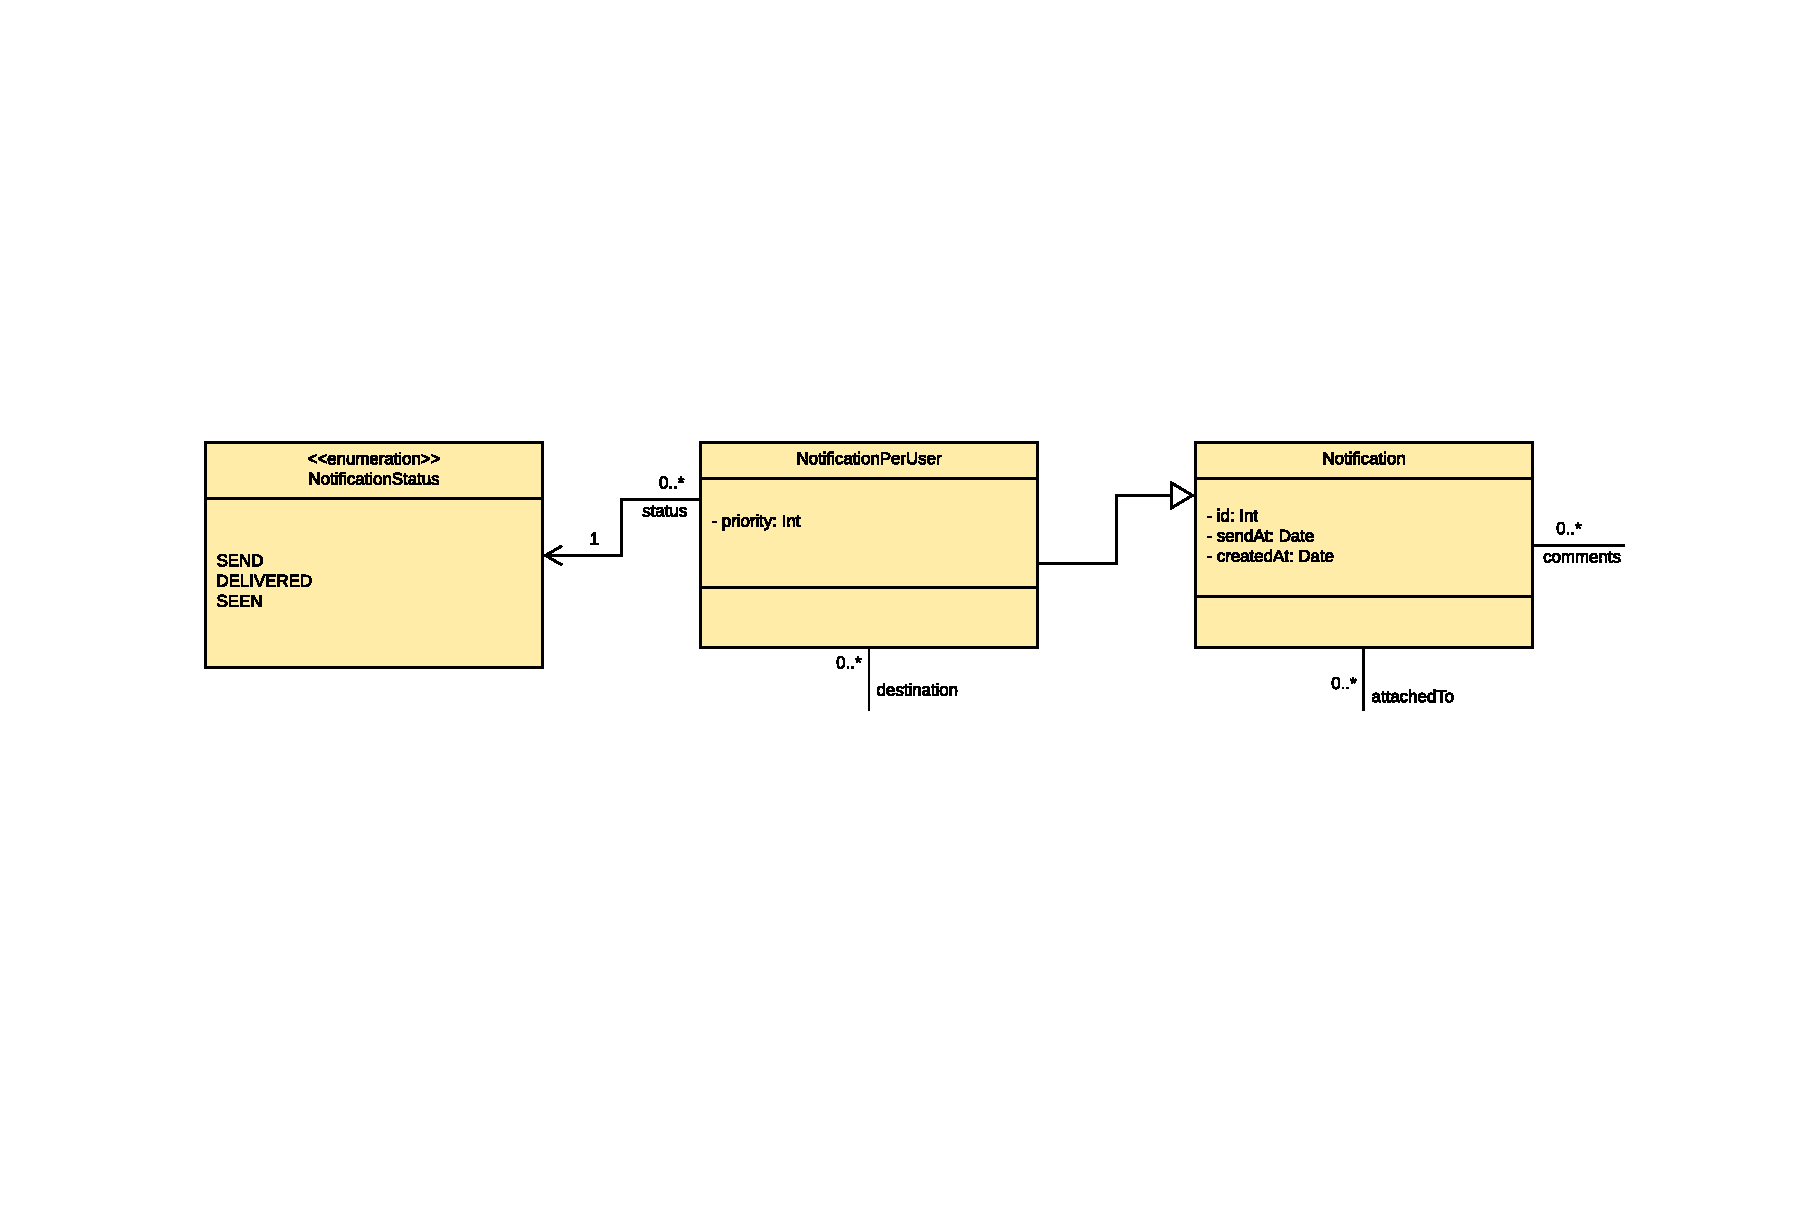
\includegraphics[angle=90, height=0.9\textheight]{pdfs/Notification1}
            \caption[Předešlý návrh oznámení]{Návrh oznámení podle doménového modelu předmětu BI-SP2}\label{image:notification1}
        \end{figure}
        \begin{figure}\centering
	        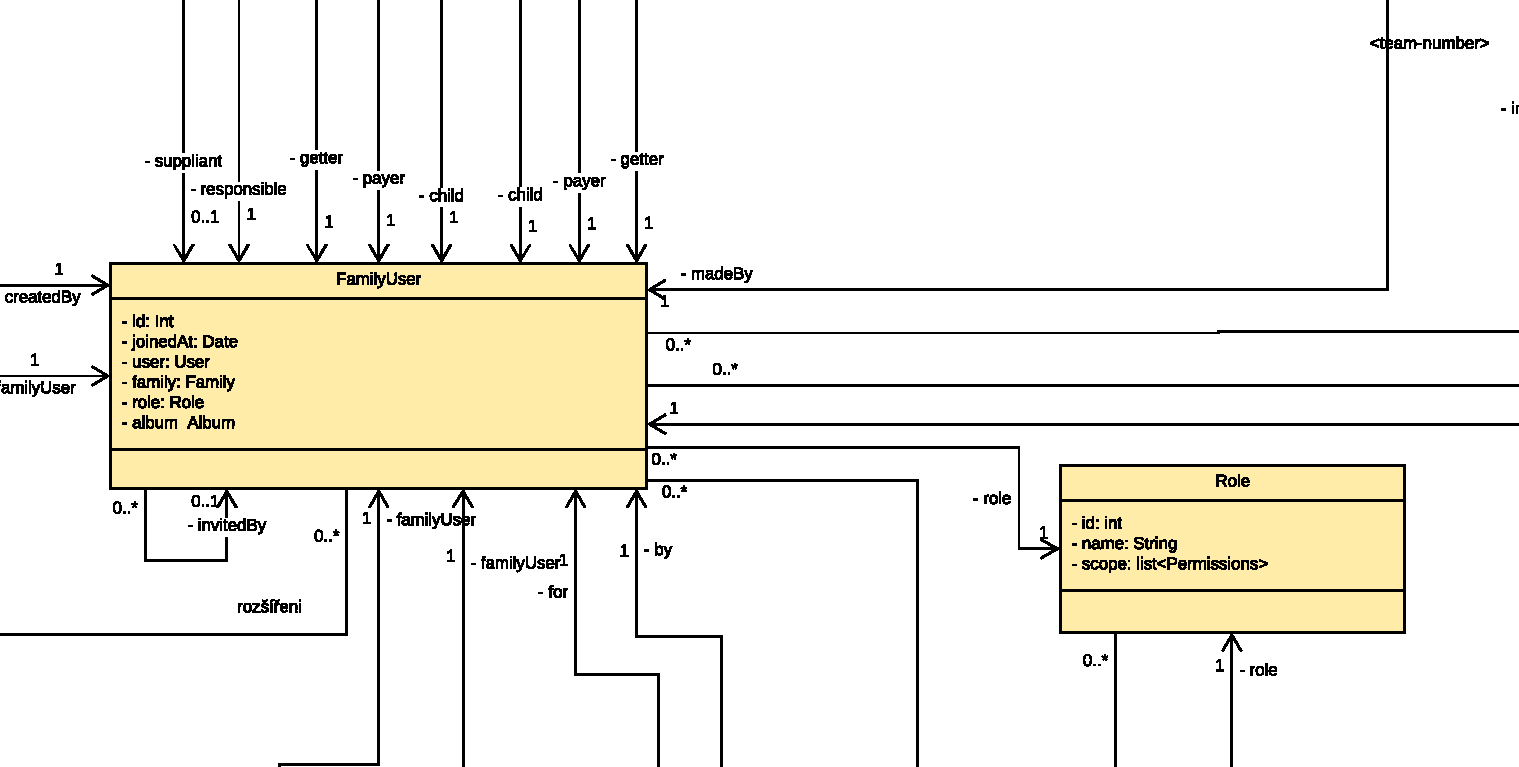
\includegraphics[angle=90, height=0.9\textheight]{pdfs/Role1}
	        \caption[Návrh \texttt{Role}]{Návrh entity \texttt{Role} podle doménového modelu z~předmětu BI-SP2}\label{image:Role1}
        \end{figure}
    % Navrh a Implementace 
    \begin{figure}\centering
	       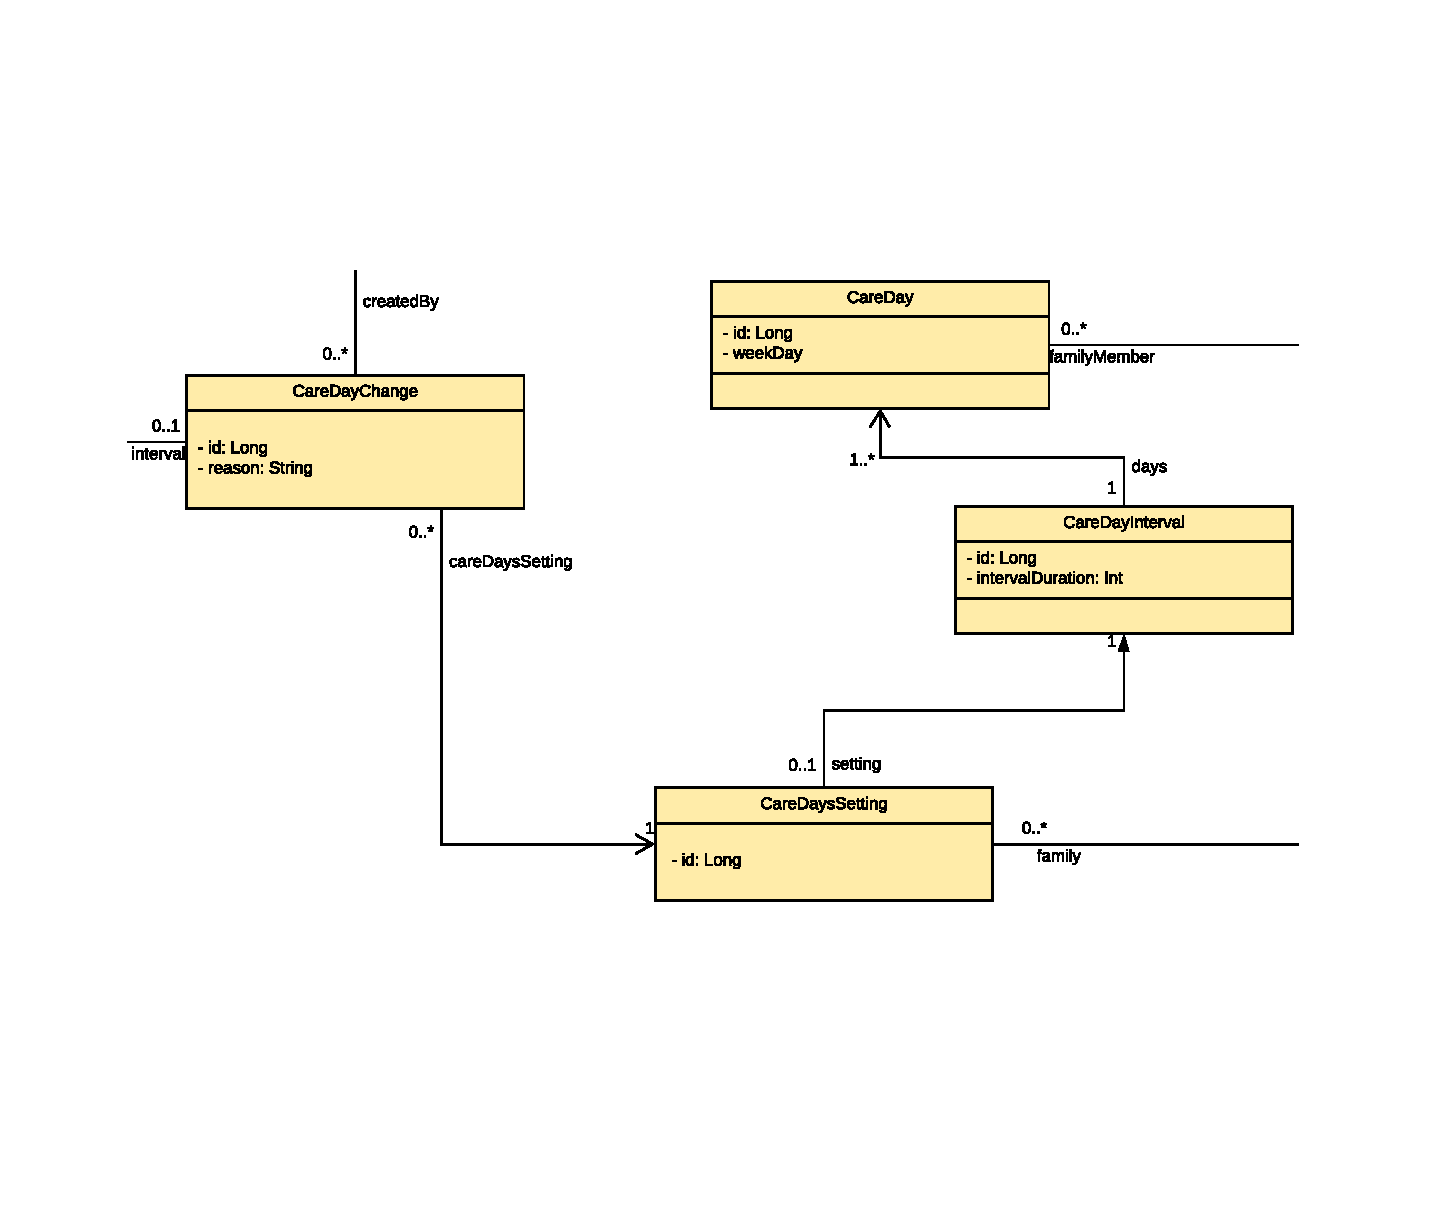
\includegraphics[angle=90, height=0.9\textheight]{pdfs/CareDays2}
	       \caption[Nový návrh pečovatelských dnů]{Nový návrh pečovatelských dnů}\label{image:caredays2}
        \end{figure}
          \begin{figure}\centering
	        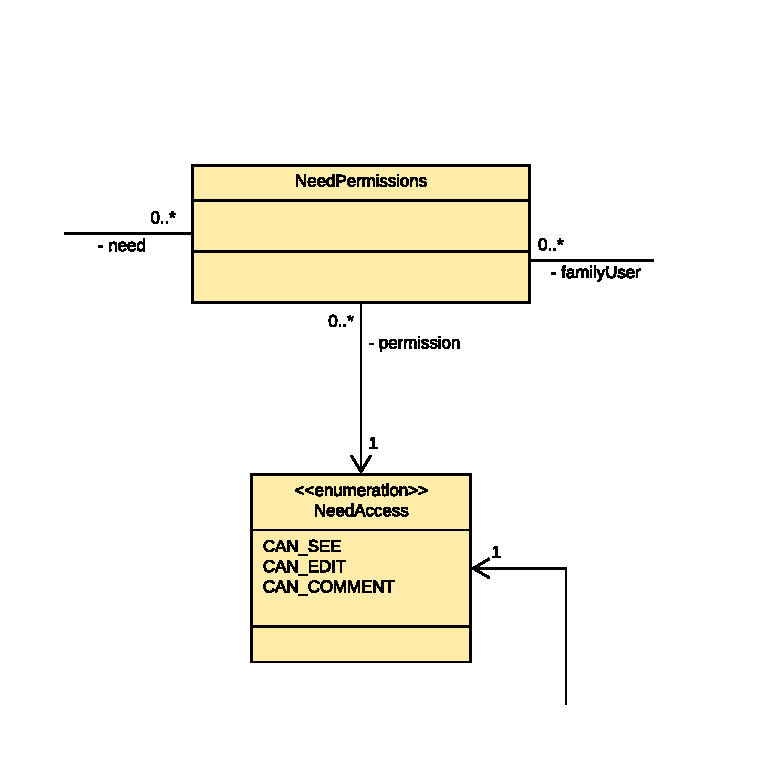
\includegraphics[width=1.0\textwidth]{pdfs/NeedPermissions1}
	        \caption[Návrh entity \texttt{NeedPermissions}]{Návrh entity \texttt{NeedPermissions} podle doménového modelu z~předmětu BI-SP2}\label{image:NeedPermissions1}
        \end{figure}
    \begin{figure}\centering
        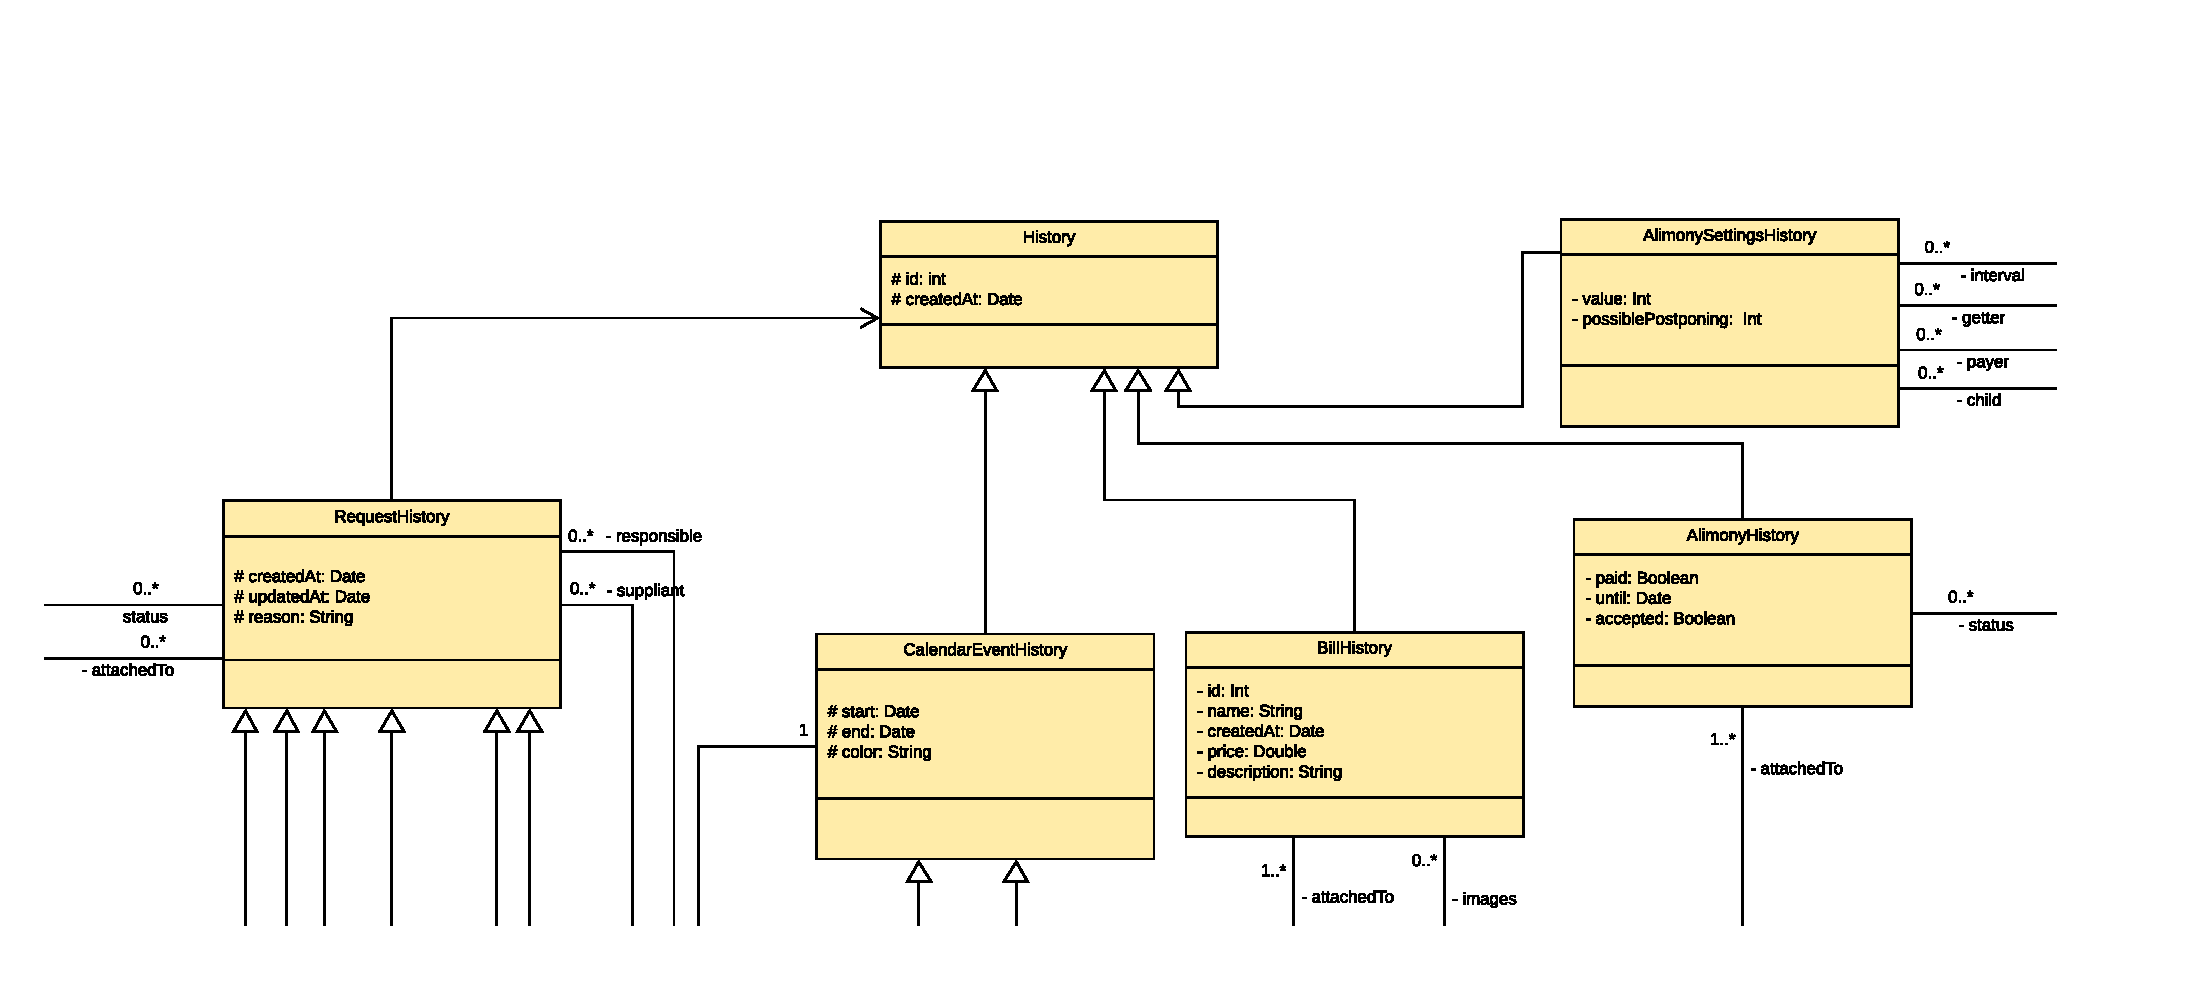
\includegraphics[angle=90, height=0.9\textheight]{pdfs/History1}
        \caption[Předešlý návrh entity \texttt{History}]{Předchozí návrh entity \texttt{History} podle doménového modelu z předmětu BI-SP2}\label{image:History1}
    \end{figure}
    \begin{figure}\centering
        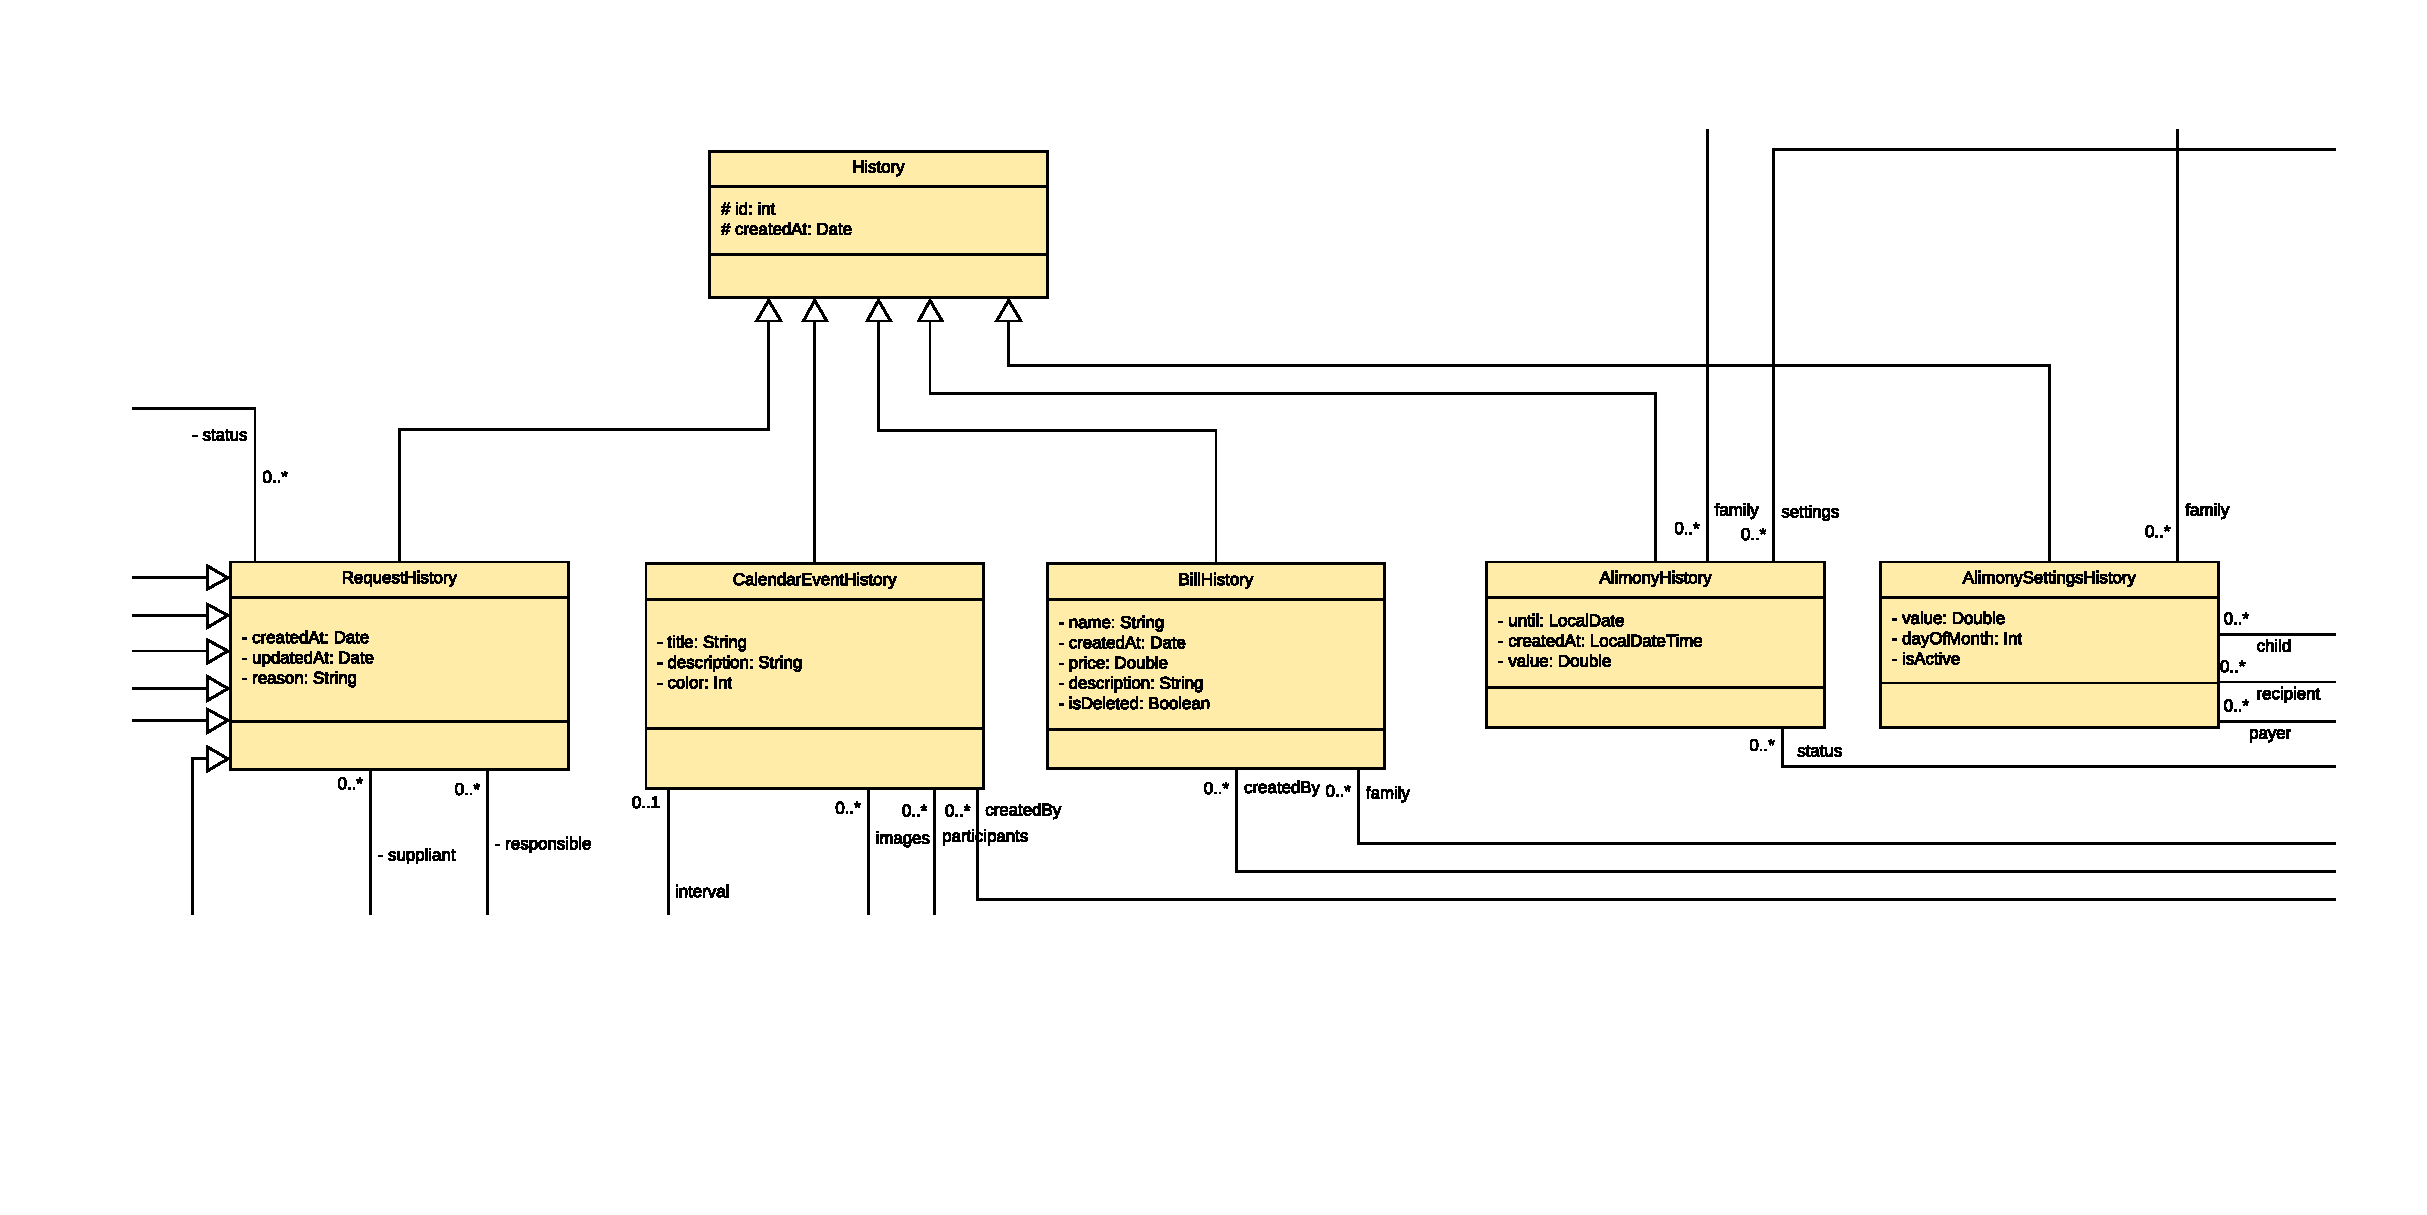
\includegraphics[angle=90, height=0.9\textheight]{pdfs/History1_2}
        \caption[Návrh entity \texttt{History} po změnách návrhu]{Návrh entity \texttt{History} po navržení změn pro entity, kterým patří příslušné entity historie}\label{image:History1_2}
    \end{figure}



%upravte podle skutecnosti

\chapter{Obsah přiloženého CD}

\begin{figure}
	\dirtree{%
		.1 README.md\DTcomment{stručný popis obsahu CD}.
		.1 jar\DTcomment{adresář se spustitelnou formou implementace}.
		.1 src.
		.2 impl\DTcomment{zdrojové kódy implementace}.
		.2 thesis\DTcomment{zdrojová forma práce ve formátu \LaTeX{}}.
		.1 text\DTcomment{text práce}.
		.2 thesis.pdf\DTcomment{text práce ve formátu PDF}.
		.2 thesis.ps\DTcomment{text práce ve formátu PS}.
	}
\end{figure}


\end{document}
